\documentclass[12pt,a4paper]{article}

% Encoding & language
\usepackage[utf8]{inputenc}

\usepackage{booktabs}
\usepackage{array}
\usepackage{float}
\usepackage{graphicx}
\usepackage{amsmath}
\providecommand{\tabularnewline}{\\}


%\usepackage[T1]{fontenc}
%\usepackage[english]{babel}


% Font Family : rmdefault is roman font
\renewcommand{\familydefault}{\rmdefault}


% Page layout & spacing
\usepackage{geometry}
\geometry{margin=1in}
\usepackage{setspace}

% 1.15 stretching
\setstretch{1.15}
\setlength{\parindent}{0pt} % Remove paragraph indentation
\setlength{\parskip}{1em} % Add space between paragraphs

% References with biblatex 
\usepackage[style=authoryear,backend=biber]{biblatex}
\addbibresource{references.bib} % your .bib file

% Hyperlinks
\usepackage[hidelinks]{hyperref}





\begin{document}
	
\title{War and Work: Labor Market Impact of the Nepalese Civil War}

\author{Suhishan Bhandari}

\date{\today}

\maketitle
	
% Section : Abstract
\begin{abstract}
	Although macro-economic consequences of Nepal's decade-long Maoist Insurgency are well-documented, macroeconomic effects remain less explored. This study examines the labor-market consequences of Nepal's Maoist Conflict using a difference-in-differences design. Variations come from a) classification of districts into high and low-conflict based on casualties, b) comparing Nepal Labour Force Survey I (1998, pre-period) with NLFS II (2008, post-period). To strengthen parallel trends, doubly-robust DiD with covariates is used. Results show that individuals in high-conflict districts were less likely to be employed and worked fewer hours post-conflict than those in low-conflict districts, with the negative employment effect strongest during rainy season. For robustness, a small sample Bayesian analysis is carried out between two adjacent districts, Gulmi and Arghakhanchi, where work hours is modeled \textit{hurdle lognormal}. The small sample result mirrors the full-sample findings.
	
	
\end{abstract}
	
	

\section{Introduction}
Nepal experienced a decade-long Civil War from 1996 to 2006 A.D. which inflicted countless injuries and claimed more than 13,000 lives \parencite{lawoti2009violent}. The Nepalese Civil War, also termed the Maoist Insurgency, was an armed struggle between the Communist Party of Nepal (Maoists) and the Nepalese Government. The conflict brought widespread destruction: damaged infrastructure, banks and industry closure, local government disruption, and conscription of young individuals into armed conflict. The paper aims to estimate the labor market implications of this violent conflict.

The literature on Maoist Insurgency has focused either on proximate causes of conflict incidence such as poverty and inequality \parencite{nepal2011more, do2010geography}, or on the effects on national GDP and tourism. The micro-economic consequences of the Nepalese Civil war, which includes effects on education and earnings, is understudied and unclear. Given the conflict's disruptive and violent nature, from adolescent conscription to the use of extreme force by the government, it is likely that economic activity, and by extension, the labor market was profoundly affected by the conflict.

The estimand in question is: \textit{How does increased conflict intensity, measured by the number of conflict-related deaths per 10,000 people, impact a person's likelihood of being employed?} While it may be reasonable to assume \textit{a priori} that conflict has a negative effect on employment, the Maoist movement's emphasis on the inclusion of marginalized communities and empowerment of women may have had a positive effect. 

I use Nepal Labor Force Survey I (NLFS I, 1998) and Nepal Labor Force Survey II (NLFS II, 2008) for individual-level data on employment, and Uppsala Conflict Data Program (UCDP) for measures on conflict casualties. To estimate the causal effect, a repeated cross-section Difference-in-Differences (DiD) approach is used, where 1998 A.D. serves as the pre-conflict period and 2008 A.D. as the post-conflict period. The analysis is restricted to districts that reported zero conflict-related casualties in 1998. A continuous treatment DiD design is adopted, since by 2008, nearly all districts in Nepal had experienced some level of conflict, leaving no truly untreated units. For the credibility of the Strong Parallel Trends (SPT) assumption, Doubly robust DiD estimator is used to control for covariates. This is different from TWFE DiD used in \textcite{menon2015war} and the conventional DiD used in \textcite{valente2014education}, two studies that have used survey data to gauge the economic consequences of the Nepalese Civil War.


Section 2 provides a brief review of the current literature on conflict causes and consequences, Section 3 sketches a simple theory linking conflict and the labor market, Section 4 describes the data and the variables used, Section 5 provides an extensive discussion on the methodology, its robustness and credibility (and absence thereof), Section 6 displays and summarizes the main results and Section 7 concludes. 

\section{Literature Review}


The first studies on conflict and economic performance used cross-country measures on prosperity like GDP and GDP per capita \parencite{blattman2010civil}. These cross country analyses have largely focused on identifying the sources of conflict, namely what factors led to the presence/absence of conflict or  variation in conflict intensity (as measured by casualties). To do so, researchers have relied on a range of theoretical frameworks including endogenous growth theory, models of information asymmetry and theories of ethno-linguistic fractionalizations. As for economic legacies, the literature has viewed evidence under two frameworks: a) The neoclassical growth theory framework which posits that conflict disrupts economic performance by affecting factors of production, technology and institutions, but implies no lasting change in equilibrium following a one-time shock; and b) Poverty Trap or endogenous growth models which suggest that conflicts can have persistent effects on future economic development.

The limited within-country micro-economic literature, which is also the scope of this paper, has relied on cross-sectional data and Difference-in-Differences method to justify causal identification of post-war legacy. \textcite{justino2013poverty} estimate that 20 percent of the Rwandan population fell into poverty following the Rwandan genocide. Using panel data on child nutrition, \textcite{alderman2006long} find that young children exposed to war-related malnutrition in Zimbabwe were significantly shorter as adults. In the context of Tajikistan, \textcite{shemyakina2011effect} reports that girls whose homes were destroyed in the civil war were less likely to obtain secondary education, with long-term domino effect on later-life wages. These results support the poverty-trap framework where exposure to conflict has affected people's long-term health, education and employment.

The literature on the Nepalese Civil War has largely followed a qualitative approach: some studies explore the conflict through a political economy perspective, underlying its role in the evolution of Nepal’s political history, while others employ ethnographic methods with small, targeted samples to test their hypotheses \parencite{lawoti2010maoist}. The first papers to prioritize large-scale empirical evidence were the papers by \textcite{bohara2006opportunity} and \textcite{do2010geography}. Their district-level analyses highlighted that the magnitude of violence depended on political and geographical opportunities for violence, for instance, mountainous terrain and dense forests. 

Building on this empirical vein, I have identified three studies that use rigorous causal methods to examine the causes and consequence of the conflict. On the causes, \textcite{nepal2011more} find that local jurisdictions in Nepal with higher inequality experienced more killings whereas poverty itself did not predict violence (in contrast to \parencite{do2010geography}). Two other studies focus on the consequences of conflict. \textcite{valente2014education} finds, counter-intuitively, that conflict casualties were associated with an increase in female educational attainment while \textcite{menon2015war} find, in a similar vein, that the likelihood of women's employment rose as a result of the conflict. While these two studies do use Difference-in-Differences, it is worth noting that the literature on DiD was not as refined as it is now. The reliance on Two way fixed effects (TWFE) with covariates by \textcite{menon2015war} for example, may not credibly identify causal effects \parencite{goodman2021difference}.


\section{Underlying Theory}
Violent conflict disrupts regional economic activity in numerous ways : destruction of infrastructure, reduced mobility, conscription of able-bodied individuals into state or rebel forces, reduced tourism due to insecurity and overall, extortion of local resources for state or rebel benefit.

Concerning the labor market, the impact of a violent conflict on regional labor market outcomes may follow two stylized paths:

\begin{enumerate}
	\item \textbf{Labor Demand Path}: During Nepal's Civil Conflict a) tourist arrival declined in Nepal, b) investment in manufacturing and service industries declined due to poor law and order, c) firms faced extortions, closures and uncertainty, and d) many banks were looted and/or destroyed \parencite{lawoti2009violent}. Additionally, the Maoists destroyed 1,683 Village Development Committees (VDC) buildings ($43\%$ of total) along with police posts, airports, electricity stations, and bridges \parencite{lawoti2009violent}. With decreasing expected returns, increase in risk, and short investment horizons, it is reasonable to expect a fall in labor demand from formal and informal employers in conflict afflicted zones. 
	
	\item \textbf{Labor Supply Path}: Civil war conscription often target school-age children, disrupting their educational and career trajectories. Post war, they may find it harder to match with potential employers. Labor supply disruption is further exacerbated by the fact that many who fight in the war are either killed or become life-long disabled. Labor Supply also may be quantitatively smaller in conflict-afflicted areas due to high volumes of emigration. An INSEC 2008 \parencite{insec2008} report details that between 2002 and 2004, $50,365$ were displaced in Nepal: $3,837$ and $21,320$ people by the state and the Maoists respectively, whereas $25,199$ persons emigrated from fear and terror.
\end{enumerate}

It is important to note that for both of these paths, an alternative income effect hypothesis is also plausible. Regarding labor demand, if local firms, in response to lower returns, offer higher wages to attract workers and stimulate economic activity in efforts for survival, conflict-afflicted zones may actually have more employment than their peaceful counterparts. In a similar vein, if displaced men are replaced by women in the workforce, or if higher wages tempt some men to stay, labor supply, again, may be higher in conflicted afflicted regions. The proposed emancipation of historically oppressed groups such as the Dalits, other socio-ethnic minorities, and women, may have had positive effects on employment by reducing discriminatory practices in the society and the workforce.



\section{Data and Variables}
This research relies on data that covers both labor market characteristics and conflict-related events in Nepal. For labor market information, I use two rounds of Nepal Labor Force Survey: NLFS 1\footnote{\url{https://microdata.nsonepal.gov.np/index.php/catalog/1/related-materials}} which was conducted in 1998 A.D. and NLFS 2\footnote{\url{https://microdata.nsonepal.gov.np/index.php/catalog/2/related-materials}} from 2008 A.D. The usage of NLFS is amenable to our analysis in two ways: 

\begin{enumerate}
	\item NLFS records detailed micro-economic data on employment: hours worked in the past 7 days, type of work a person is involved in, reasons for inactivity, any education or training received and other key variables pertinent to labor market analysis.
	
	\item The NLFS is a nationally representative survey, with large sample sizes obtained through a two-stage stratified sampling procedure based on Probability Proportional to Size (PPS). 
\end{enumerate}

Labor Market data from NLFS is merged with conflict-event data from Uppsala Conflict Data Program (UCDP), collected and maintained by Uppsala University, Sweden\footnote{\url{https://ucdp.uu.se/}}. UCDP provides detailed and timed records of all casualties with Geo-spatial information on the district of incidence, number of deaths (with lower and upper bound estimates), who died – Maoists, civilians or the police officials, and the dyadic context of the conflict i.e. who initiated the conflict as reported by the source.

Since the main variable of interest is work, the definition and scope of what is deemed work must be clear, especially in a developing economy like Nepal. The scope of work in NLFS is based on ILO standards and 1993 System of National Accounts (SNA). The example of activities which count as work include: wage job, any business operated by the person, agriculture, milling and other food processing, handicrafts, construction and major repairs, fetching water, collecting firewood, and other work activities\footnote{For more detail, see NLFS I or NLFS II Report's section on Work.}. A key caveat in classifying work activities involves the inclusion of tasks such as collecting firewood and fetching water. In rural Nepal, where a significant share of the population must perform these tasks for household survival, extending the production boundary to count these activities as employment may distort labor market estimates. All work-related measures in this paper exclude people \textit{exclusively} involved in collecting firewood and fetching water.


\begin{table}[H]
	\caption{Variables and Description}
	
	\renewcommand{\arraystretch}{1.2}
	
	\begin{tabular}{|>{\centering}p{5cm}|>{\centering}p{10cm}|}
		\hline 
		Variable & Description\tabularnewline
		\hline 
		\hline 
		Usually Employed  & A person is assumed usually employed when they have worked more than
		180 days (NLFS I) or more than or equal to 6 full months (NLFS II)\tabularnewline
		\hline 
		Currently Employed  & There are two situations in which a person can be defined as being
		currently employed. Either the person is actually working in the reference
		week (here the last 7 days), or he or she has an attachment to a job
		or business but did not work during the reference week.\tabularnewline
		\hline 
		Currently Self Employed  & As a subset of currently employed, a person is currently self-employed
		if she fulfills working in the categories of work defined unde the
		self-employment category such as agriculture, handicraft, food processing
		at home for sale, etc.\tabularnewline
		\hline 
		Work Hours (cont) & The number of hours worked in the last 7 days.\tabularnewline
		\hline 
		Work Hours -- Self Emp (cont) & The number of self employment hours in the last 7 days.\tabularnewline
		\hline 
		Conflict Deaths (cont) & From the UCDP dataset, the best estimate of the number of people that
		died in a conflict between Maoist Insurgents and the Government of
		Nepal between 1996 and 2006 A.D. (for every district)\tabularnewline
		\hline 
		Conflict Deaths per 10000 population (cont) & Conflict Deaths standardized to population of every district (population
		metrics from Nepal's 2001 Census)\tabularnewline
		\hline 
		Age (cont) & Age of the people surveyd\tabularnewline
		\hline 
		Ever Attented School  & A categorical variable indicating whether the person surveyed ever
		attended school.\tabularnewline
		\hline 
		Year of education (cont) & Total years of completed years of schooling, among those who did attend
		school i.e. among ever attended school = 1.\tabularnewline
		\hline 
		Years of education for all (cont) & Completed Years of schooling whereby those who never attended school
		are coded as 0.\tabularnewline
		\hline 
		Hindu  & If a person surveyed identifies as Hindu.\tabularnewline
		\hline 
		Brahmin/Chhetri  & If a person surveyed belongs to either Brahmin or Chhetri Caste i.e.
		the privileged class.\tabularnewline
		\hline 
		Male  & If a person is male.\tabularnewline
		\hline 
		Married  & A variable indicating whether a person is currently married.\tabularnewline
		\hline 
		Household Size & The size of the household that a person belongs to. Members from the
		same household have the same household size.\tabularnewline
		\hline 
		Urban & Whether a person's household resides in an urban or a rural area.\tabularnewline
		\hline 
	\end{tabular}
\end{table}
\begin{table}
	
	\caption{Table of Summary Statistics}
	
	\renewcommand{\arraystretch}{1.5}
	
	\begin{tabular}{lcccc}
		& Mean & SD & Min & Max\tabularnewline
		\hline 
		Usually Employed  & 0.71 & 0.45 & 0 & 1\tabularnewline
		Currently Employed  & 0.73 & 0.44 & 0 & 1\tabularnewline
		Currently Self Employed  & 0.57 & 0.50 & 0 & 1\tabularnewline
		Work Hours  & 31.94 & 25.3 & 0 & 84\tabularnewline
		Self Employed Work Hours & 22.42 & 24.8 & 0 & 84\tabularnewline
		Conflict Deaths  & 109 & 65.4 & 26 & 328\tabularnewline
		Conflict Deaths per 10000 population  & 5.57 & 4.7 & 0.832 & 22.2\tabularnewline
		Age (cont) & 31.56 & 12.02 & 15 & 59\tabularnewline
		Ever Attended School  & 0.58 & 0.49 & 0 & 1\tabularnewline
		Year of education (cont) & 8.72 & 3.81 & 0 & 18\tabularnewline
		Years of education for all (cont) & 5.73 & 5.17 & 0 & 18\tabularnewline
		Hindu  & 0.85 & 0.36 & 0 & 1\tabularnewline
		Brahmin/Chhetri & 0.33 & 0.47 & 0 & 1\tabularnewline
		Male  & 0.47 & 0.5 & 0 & 1\tabularnewline
		Married  & 0.70 & 0.46 & 0 & 1\tabularnewline
		Household Size & 5.65 & 2.69 & 1 & 29\tabularnewline
		Urban & 0.57 & 0.49 & 0 & 1\tabularnewline
		\hline 
	\end{tabular}
	
\end{table}


\section{Empirical Method}
This paper employs Difference-in-Difference to gauge the causal impact of Nepal's Maoist Civil War on the likelihood of employment. Let $Y$ denote whether an individual is usually employed, and $D$ denote treatment status (1 if treated, 0 otherwise), where treatment is based on the level of conflict-related casualties in a given district \footnote{The mechanism behind treatment assignment is explained in the following section}. Let $t=1$ and $t=2$ represent the pre-period of 1998 A.D. and post-period of 2008 A.D respectively. Under the standard parallel trends assumption, the canonical DiD framework estimates the Average Treatment Effect on the Treated (ATT) as:
\begin{equation}
	ATT=(E[Y_{i,t=2}|D=1]-E[Y_{i,t=1}|D=1])-(E[Y_{i,t=2}|D=0]-E[Y_{i,t=1}|D=0])
\end{equation}

While the canonical DiD setup serves as a useful tool for preliminary analysis, estimating $ATT$ in this empirical context requires much stronger assumptions and more appropriate estimators. The limitations of the standard approach along with the proposed methodological adjustments is discussed in the subsections that follow.

\subsection{Classification into Treatment and Control}
There are two major difficulties in classifying Nepal's districts into conflicted-afflicted (treatment) and not-conflict-afflicted (control) groups:

\begin{enumerate}
	\item The first concern pertains to the use of 1998 Nepal Labor Force Survey (NLFS 1) as the pre-treatment period. Since the Civil War began in 1996, several districts had already experienced substantial conflict-related casualties by 1998.
	
	\item By the end of the conflict in 2008, very few districts (e.g. Manang and Mustang) remained untouched by violence. Nearly all districts had experienced some degree of conflict, which the literature refers as no untreated units classification.
	
\end{enumerate}

I attend to the concerns in the following ways\footnote{The following subsection is highly influenced by \parencite{callaway2024difference}. Please refer to it for further exposition and explanation}



\begin{enumerate}
	\item I filter the sample to only those districts that had 0 conflict casualties up until the end of 1998 A.D. This limits the sample to 38 districts. (Districts like Manang and Mustang are excluded in the analysis.)
	
	\item Given that conflict intensity, measured as conflict casualties per population, is a continuous metric, the canonical DiD non-parametric estimator for $ATT$ must be adapted to\footnote{I follow the conventional potential outcomes framework as outlines in \parencite{baker2025difference} and use similar notation. For notational reference, please check this paper.}:
	\begin{equation}
		E[\Delta Y|D=d_{H}]-E[\Delta Y|D=d_{L}]=ATT(d_{H}|d_{H})-ATT(d_{L}|d_{L})
	\end{equation}
	\begin{enumerate}
		\item This specification compares the outcome evolution of districts exposed to high treatment intensity $d_H$ with those exposed to the lowest observed treatment intensity $d_L$, since no districts remained entirely untreated. The estimator captures the average causal effect of moving from $d_L$ to $d_H$, but includes a potential selection bias term. That is, it assumes that the change in outcomes for units with treatment $d_L$ serves as the valid counterfactual for those with higher treatment $d_H$. This is a much stronger assumption than in binary-treatment DiD designs and requires invoking Strong Parallel Trends (SPT) \parencite{callaway2024difference}. Under strong parallel trends we have:
		
		\begin{equation}
			E[\Delta Y|D=d_{H}]-E[\Delta Y|D=d_{L}]=E[Y_{t=2}(d_{H})-Y_{t=2}(d_{L})|D>0]
		\end{equation}
		
		\item The SPT assumes that lower dose groups are valid counterfactuals for higher dose groups. While this is a strong assumption, the plausibility of SPT can be improved by conditioning on observed covariates $X$.
	\end{enumerate}
	
	If these arguments are summarized and constellated, we can estimate Average Treatment Effect on the treated (ATT) in our empirical context as:
	
	\begin{equation}
		ATT_{x}(d_{H})=E[Y_{t=2}(d_{H})-Y_{t=2}(d_{L})|X=x,D>0]
	\end{equation}
	
	As noted earlier, the empirical design follows what the DiD literature refers to as a no untreated units specification. In this setup, I compare units that are “more treated” ($d_H$) to units that are “less treated”($d_L$). This is evidenced from table 3, where differences in the dose of treatment (here, conflict-related deaths per 10000 population) is shown. Districts with conflict casualty rates above the 75th percentile are classified as “more treated” (treatment group), while those below this threshold are considered “less treated” (control group). The regression results in table 4 indicate that, under this classification, more-treated districts experienced conflict casualties that were $1.8$ standard deviations higher than those in less-treated districts\footnote{Conflict casualties per 10,000 population is used instead of raw conflict casualties information to relativize the magnitude of the impact of conflict. This is done because high death toll in a highly populated district and high death toll in a lowly populated district do not signify the same impact.}.

\end{enumerate}
	
	% Conflict Intensity Table
	\begin{table}[H]
		\caption{d and $d_{L}$ i.e High and Low-dose groups conflict intensity}
		
		\renewcommand{\arraystretch}{1.2}
		\vspace{1em}
		\centering{}
			\begin{tabular}{c|c|c}
				& 1998 (pre-period) & 2008 (post-period)\tabularnewline
				\hline 
				$E[D = d_{L}]$ & $0$ & $3.34$\tabularnewline
				$E[D = d_{H}]$ & $0$ & $11.8$\tabularnewline
				\hline 
			\end{tabular}
			
		\vspace{1em}
		
		Note: The values in the table are Conflict Deaths between 1996 and
		2008 per 10,000 population (population metrics from 2001 Census)
	\end{table}
	
	% Sample Size Classification
	\begin{table}[H]
		\caption{Sample Size Classification}
		
		\renewcommand{\arraystretch}{1.2}
		\vspace{1em}
		\centering{}%
		\begin{tabular}{c|c|c}
			& 1998 (pre-period) & 2008 (post-period)\tabularnewline
			\hline 
			$E[D = d_{L}]$ & $18,660$ & $22,618$\tabularnewline
			$E[D = d_{H}]$ & $1287$ & $1756$\tabularnewline
			\hline 
		\end{tabular}
	\end{table}
	
	
% Table created by stargazer v.5.2.3 by Marek Hlavac, Social Policy Institute. E-mail: marek.hlavac at gmail.com
% Date and time: Fri, Sep 19, 2025 - 11:58:01 AM
\begin{table}[!htbp] \centering 
  \caption{Conflict Deaths per 10,000 population regressed on Treatment Status} 
  \label{} 
\begin{tabular}{@{\extracolsep{5pt}}lc} 
\\[-1.8ex]\hline 
\hline \\[-1.8ex] 
 & \multicolumn{1}{c}{\textit{Dependent variable:}} \\ 
\cline{2-2} 
\\[-1.8ex] & Conflict Deaths per 10,000 population (std) \\ 
\hline \\[-1.8ex] 
 Treatment (1/0) & 1.803 \\ 
  & (0.222) \\ 
  & \\ 
 Constant & $-$0.475 \\ 
  & (0.114) \\ 
  & \\ 
\hline \\[-1.8ex] 
Observations & 38 \\ 
R$^{2}$ & 0.648 \\ 
Adjusted R$^{2}$ & 0.638 \\ 
\hline 
\hline \\[-1.8ex] 
\textit{Note:}  & \multicolumn{1}{r}{(std) represents standardized variables} \\ 
\end{tabular} 
\end{table} 

	
	
\begin{figure}[H]
	\centering
	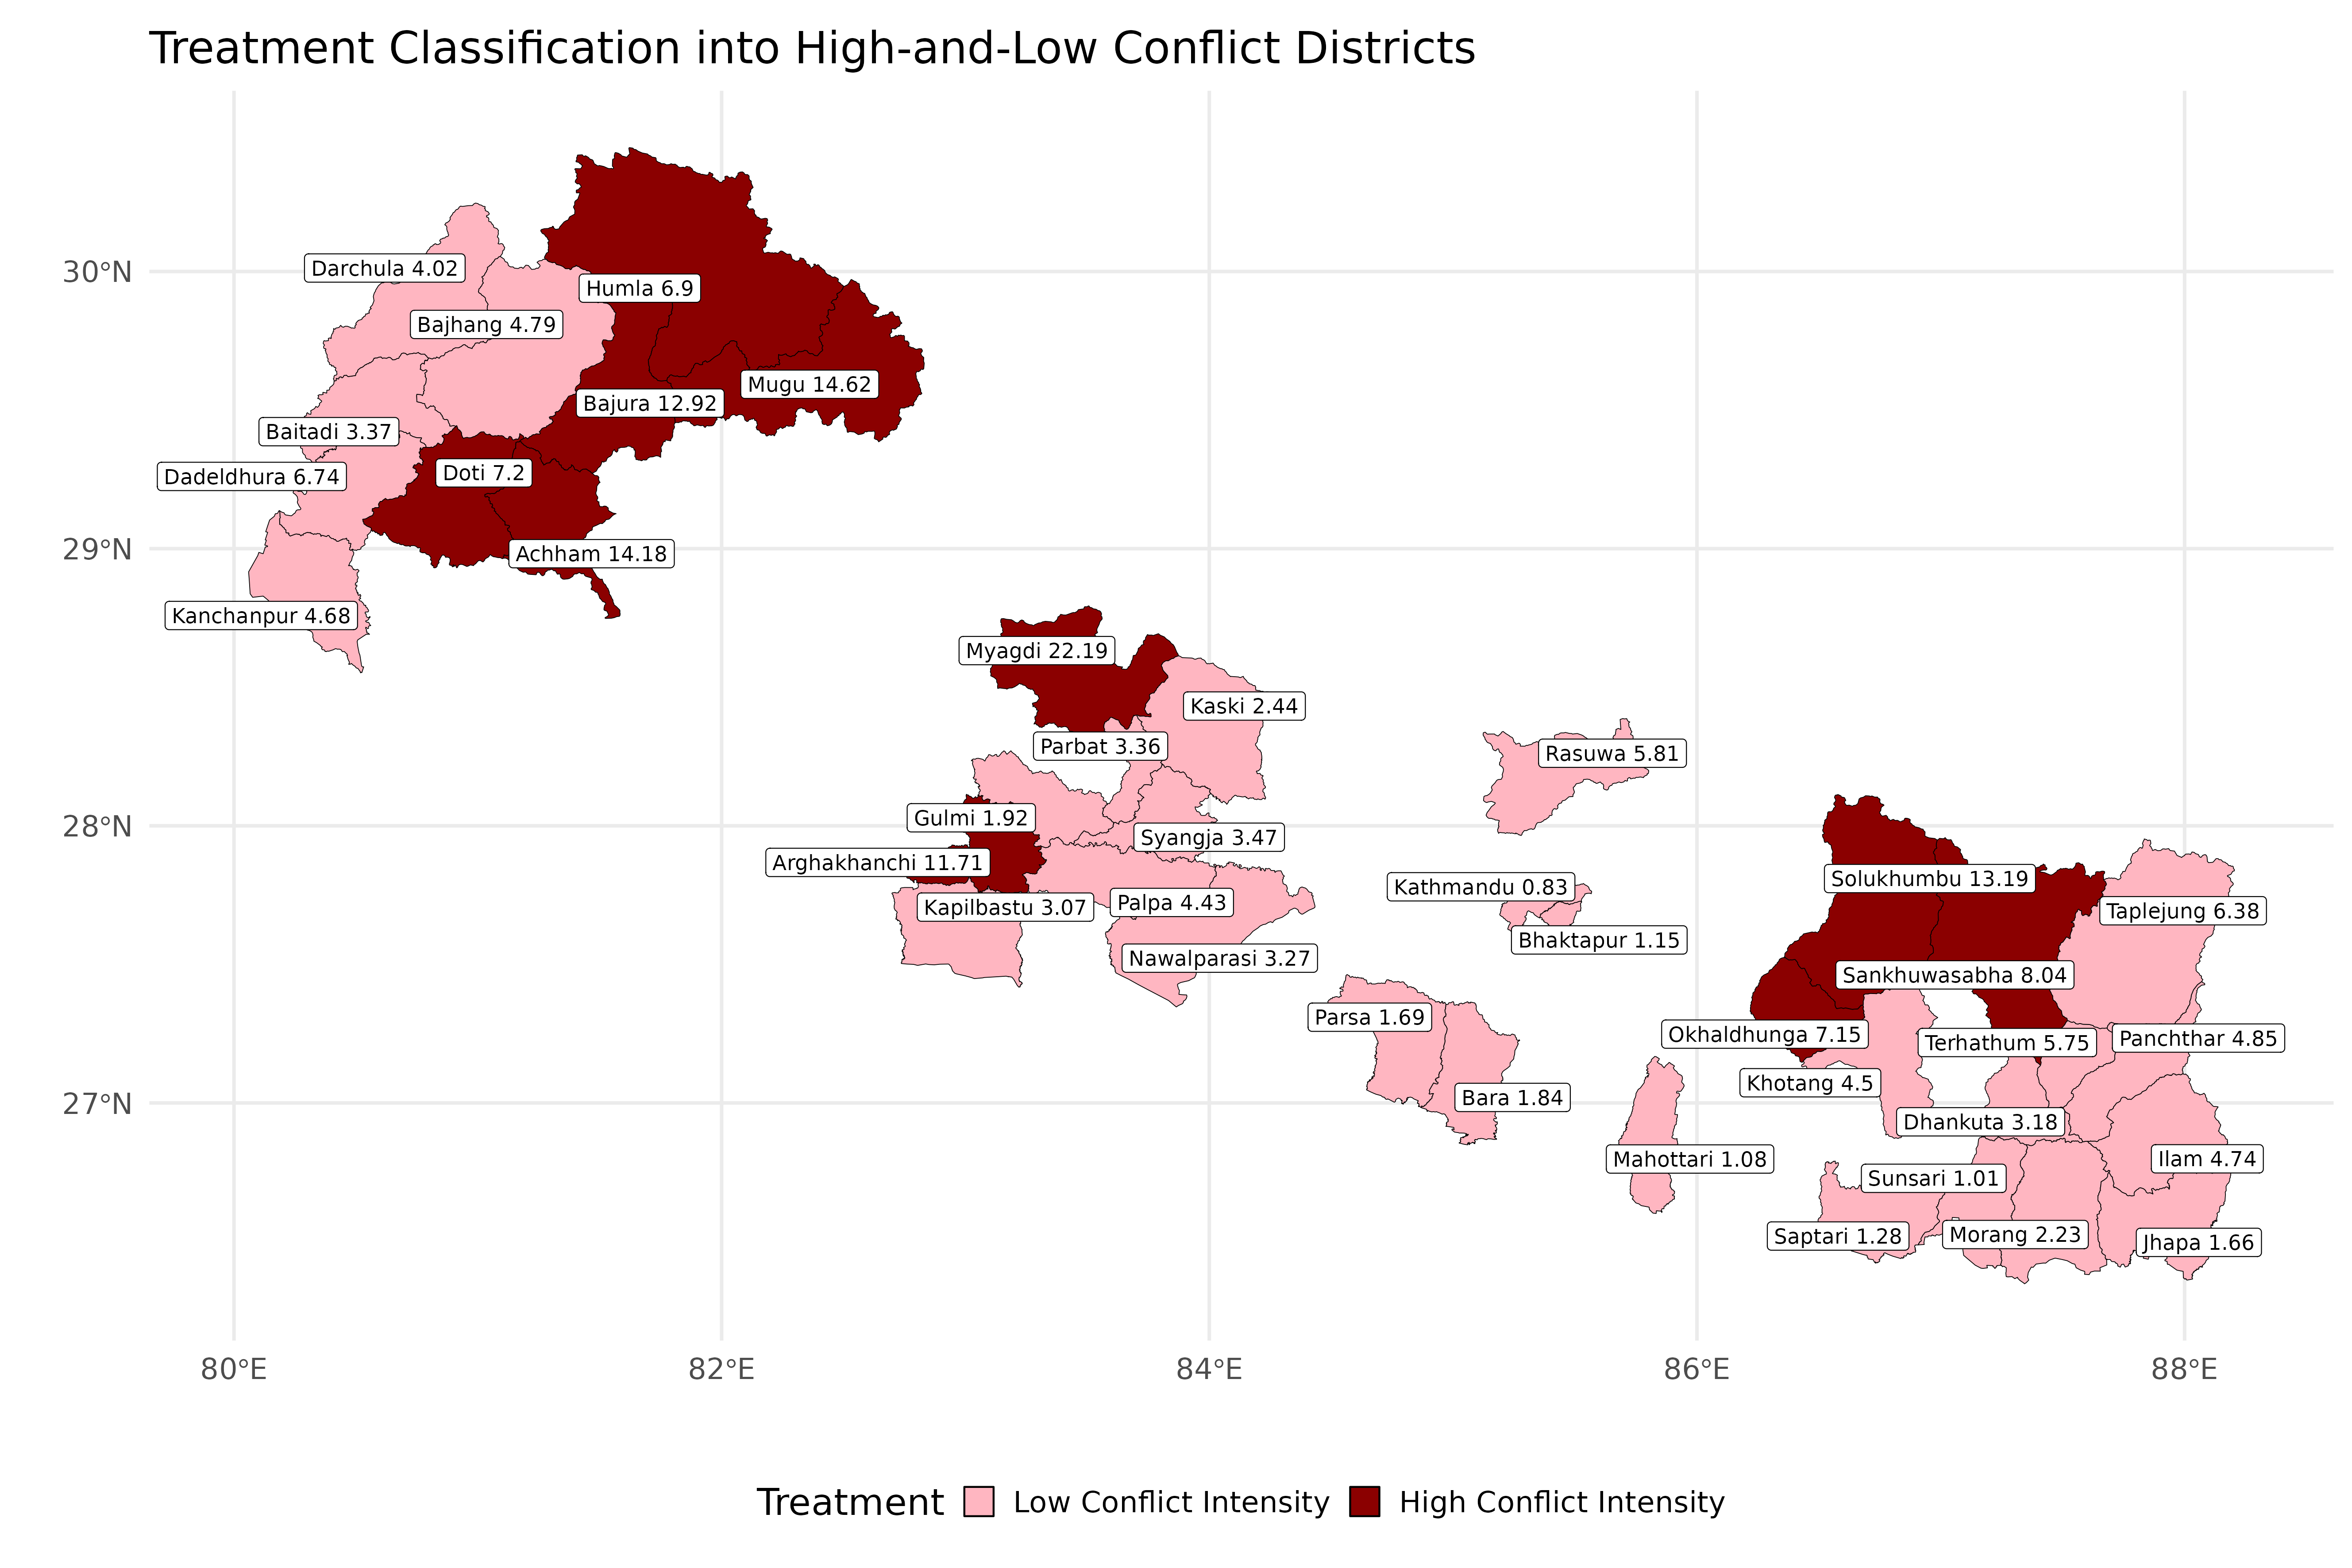
\includegraphics[width=1\textwidth]{../Analysis files/overall_conflict_map.png}
	\caption{The figure shows the categorization of districts into high-conflict (dark red) and low-conflict (light pink) districts. Districts are labeled with their measures of conflict casualties per 10,000 population.}
	\label{fig:overall_conflict_map}
\end{figure}

\subsection{Strong Parallel Trends and DiD with Covariates}
In the previous section, I noted that estimating the causal effect of conflict intensity (as proxied by conflict-related deaths) on employment requires strengthening the parallel trends assumption. Specifically, this implies that districts with lower conflict intensity (low-dose) must serve as valid counterfactuals for districts with higher conflict intensity (high-dose). However, this assumption becomes implausible if these two groups differ systematically in observable characteristics that influence employment outcomes. For eg: let's suppose that during 1998 A.D. (the pre-period), individual employment status was strongly associated with years of education or ethnic background. If this relationship would've persisted in low-conflict areas, and if highly-afflicted and low-afflicted districts differ along these dimensions, then the parallel trends assumption may fail to hold. In such a case, the observed trends in low-afflicted districts cannot serve as untreated potential outcome for highly afflicted districts. Therefore, as emphasized by \parencite{baker2025difference}, checking balance in observable determinants of $Y_i,t(d_L)$ is a sensible way to evaluate the validity of parallel trends (in this case strong parallel trends).

I assess for balance in the following variables : a person' age, years of education, whether a person is Hindu, whether a person belongs to Brahmin/Chhetri ethnicity, a person's sex, marital status, household size and whether the person lived in an urban or rural area. Table 6 presents group-wise averages for these variables in 1998 A.D. along with their normalized differences\footnote{Norm Diff = $\frac{{\bar{X}_{T}-\bar{X}_{C}}}{\sqrt{0.5(SD_{T}^{2}+SD_{C}^{2})}}$}.

% latex table generated in R 4.1.2 by xtable 1.8-4 package
% Thu Sep 18 16:11:13 2025
\begin{table}[ht]
\centering
\begin{tabular}{rrrr}
  \toprule
 & Norm. Diff & Treated Mean & Control Mean \\ 
  \midrule
Age & 0.03 & 31.73 & 31.38 \\ 
  Years of Education (All) & -0.68 & 2.31 & 5.23 \\ 
  Years of Education (If attended school) & -0.74 & 6.07 & 8.45 \\ 
  Hindu (1/0) & 0.18 & 0.92 & 0.86 \\ 
  Brahmin/Chhetri(1/0) & 0.43 & 0.54 & 0.33 \\ 
  Male & -0.15 & 0.41 & 0.49 \\ 
  Married & 0.04 & 0.73 & 0.71 \\ 
  Household Size & -0.14 & 5.44 & 5.76 \\ 
  Urban & -0.94 & 0.18 & 0.60 \\ 
  Ever Attended School & -0.49 & 0.38 & 0.62 \\ 
   \bottomrule
\end{tabular}
\caption{Covariate Balance Statistics} 
\end{table}


There are meaningful imbalances in several baseline (pre-period) variables. \textcite{imbens2015causal} suggest that a normalized difference exceeding $|0.25|$ indicates substantive imbalance between treatment and control groups. According to this heuristic, highly afflicted and less afflicted regions differed in completed years of education, if they ever attended school, composition of Hindus and Brahmin/Chhetris, as well as urban/rural residency. This imbalance highlights two important points:	
\begin{enumerate}
	\item Conflict incidence is probably not exogenous. There are systematic differences in pre-conflict observable characteristics like education, ethnic composition and rurality, which may predict conflict incidence.
	
	\item There is a risk of parallel trends violation if areas starting out with different education level or ethnic composition would have followed different employment trends in conflict's absence.
\end{enumerate}

Another way to assess imbalance between high and low conflict afflicted regions is by examining changes in observable characteristics over time. Table 7 shows the 1998-2008 trend for some observable covariates. 


% latex table generated in R 4.1.2 by xtable 1.8-4 package
% Fri Sep 19 11:58:01 2025
\begin{table}[ht]
\centering
\begin{tabular}{rrr}
  \toprule
 & Control trend & Treatment trend \\ 
  \midrule
Age & 0.28 & 0.33 \\ 
  Years of Education (All) & 1.23 & 1.91 \\ 
  Years of Education (If attended school) & 0.64 & 1.31 \\ 
  Hindu (1/0) & -0.02 & -0.05 \\ 
  Brahmin/Chhetri(1/0) & -0.02 & -0.07 \\ 
  Male & -0.02 & 0.02 \\ 
  Married & -0.02 & -0.01 \\ 
  Household Size & -0.20 & 0.51 \\ 
  Urban & 0.01 & -0.02 \\ 
  Ever Attended School & 0.09 & 0.19 \\ 
   \bottomrule
\end{tabular}
\caption{Covariate Balance Statistics for trends/differences (2008 - 1998)} 
\end{table}


As with baseline covariates, there are some meaningful differences in trends. For instance, more-afflicted districts saw greater increases in completed years of schooling and school attendance. Household size also rose in treated districts, while it declined in controls. Trend imbalance is useful if differences are meaningful contributors to untreated (here less-treated) potential outcomes $\Delta Y_{i,t}(d_{L})$. For example, it is plausible that increase in completed years of schooling may affect employment. As such, using such a variable as a covariate seems sensible. However, if covariate itself is influenced by treatment, controlling for it may bias the estimate. This is true for educational measures, which were likely influenced by conflict, and its inclusion may introduce bias. In summary, while exogenous covariate changes may indicate a violation of parallel trends, change in endogenous covariates may reflect a consequence of the treatment itself, and as such may not be appropriate controls.


\subsection{Estimator: Doubly Robust DiD}

A useful way to account for covariate imbalances is the doubly robust DiD estimator from \parencite{sant2020doubly}. This estimator uses both outcome-regression (regression adjustment, RA) and Inverse Probability Weighting (IPW) approaches. In the outcome regression approach, outcome changes for untreated units (here, less-treated) are regressed on covariates, and the fitted model thus achieved is use to predict treated units' trends. This provides a counterfactual trend for treated units, which is then subtracted from the actual trend to get the treatment effect. 

The IPW procedure, on the other hand, models treatment assignment on observed covariates, obtains propensity scores for the probability of being treated, and re-weights the changes in outcome to ensure that treatment and control groups are similar on covariates.

In our context, it is both equally plausible that imbalance in urban status, sex, religion and ethnicity in 1998 A.D. affects employment trends and how such imbalances are the reason some have higher conflict intensity than others. The former concern is addressed by RA and the latter is dealt by IPW. The doubly robust DiD accounts for both such potential violations of parallel trends, and offers protection even if either one of the model is misspecified\footnote{For more on Doubly Robust methods, with practical examples and good intuition, see \textcite{baker2025difference}}.


Table 8 presents the results from the propensity score model, showing that covariates such as ethnicity, sex, and urban/rural status are strong predictors of exposure to high-conflict intensity. The corresponding overlap in estimated propensity scores is displayed in Figure 1, where we can see good common support and overlap between treated and control groups. This overlap suggests that treatment and control groups are sufficiently comparable, and we can make meaningful inferences from the Doubly robust DiD estimates in Section 6.


% Table created by stargazer v.5.2.3 by Marek Hlavac, Social Policy Institute. E-mail: marek.hlavac at gmail.com
% Date and time: Thu, Sep 18, 2025 - 04:11:14 PM
\begin{table}[!htbp] \centering 
  \caption{Propensity Score Regression on observed covariates (1998 NLFS)} 
  \label{} 
\begin{tabular}{@{\extracolsep{5pt}}lc} 
\\[-1.8ex]\hline 
\hline \\[-1.8ex] 
 & \multicolumn{1}{c}{\textit{Dependent variable:}} \\ 
\cline{2-2} 
\\[-1.8ex] & Treatment (high-conflict) \\ 
\hline \\[-1.8ex] 
 Hindu & $-$0.317 \\ 
  & (0.508) \\ 
  & \\ 
 Brahmin/Chhetri & 0.542$^{*}$ \\ 
  & (0.287) \\ 
  & \\ 
 Sex & $-$0.197$^{***}$ \\ 
  & (0.057) \\ 
  & \\ 
 Poverty Rate & 0.048$^{***}$ \\ 
  & (0.012) \\ 
  & \\ 
 Urban & $-$1.345$^{**}$ \\ 
  & (0.530) \\ 
  & \\ 
 Constant & $-$3.944$^{***}$ \\ 
  & (0.726) \\ 
  & \\ 
\hline \\[-1.8ex] 
Observations & 19,902 \\ 
Log Likelihood & $-$3,719.054 \\ 
Akaike Inf. Crit. & 7,450.108 \\ 
\hline 
\hline \\[-1.8ex] 
\textit{Note:}  & \multicolumn{1}{r}{Standard errors are psu-clustered} \\ 
\end{tabular} 
\end{table} 


\begin{figure}[H]
\centering
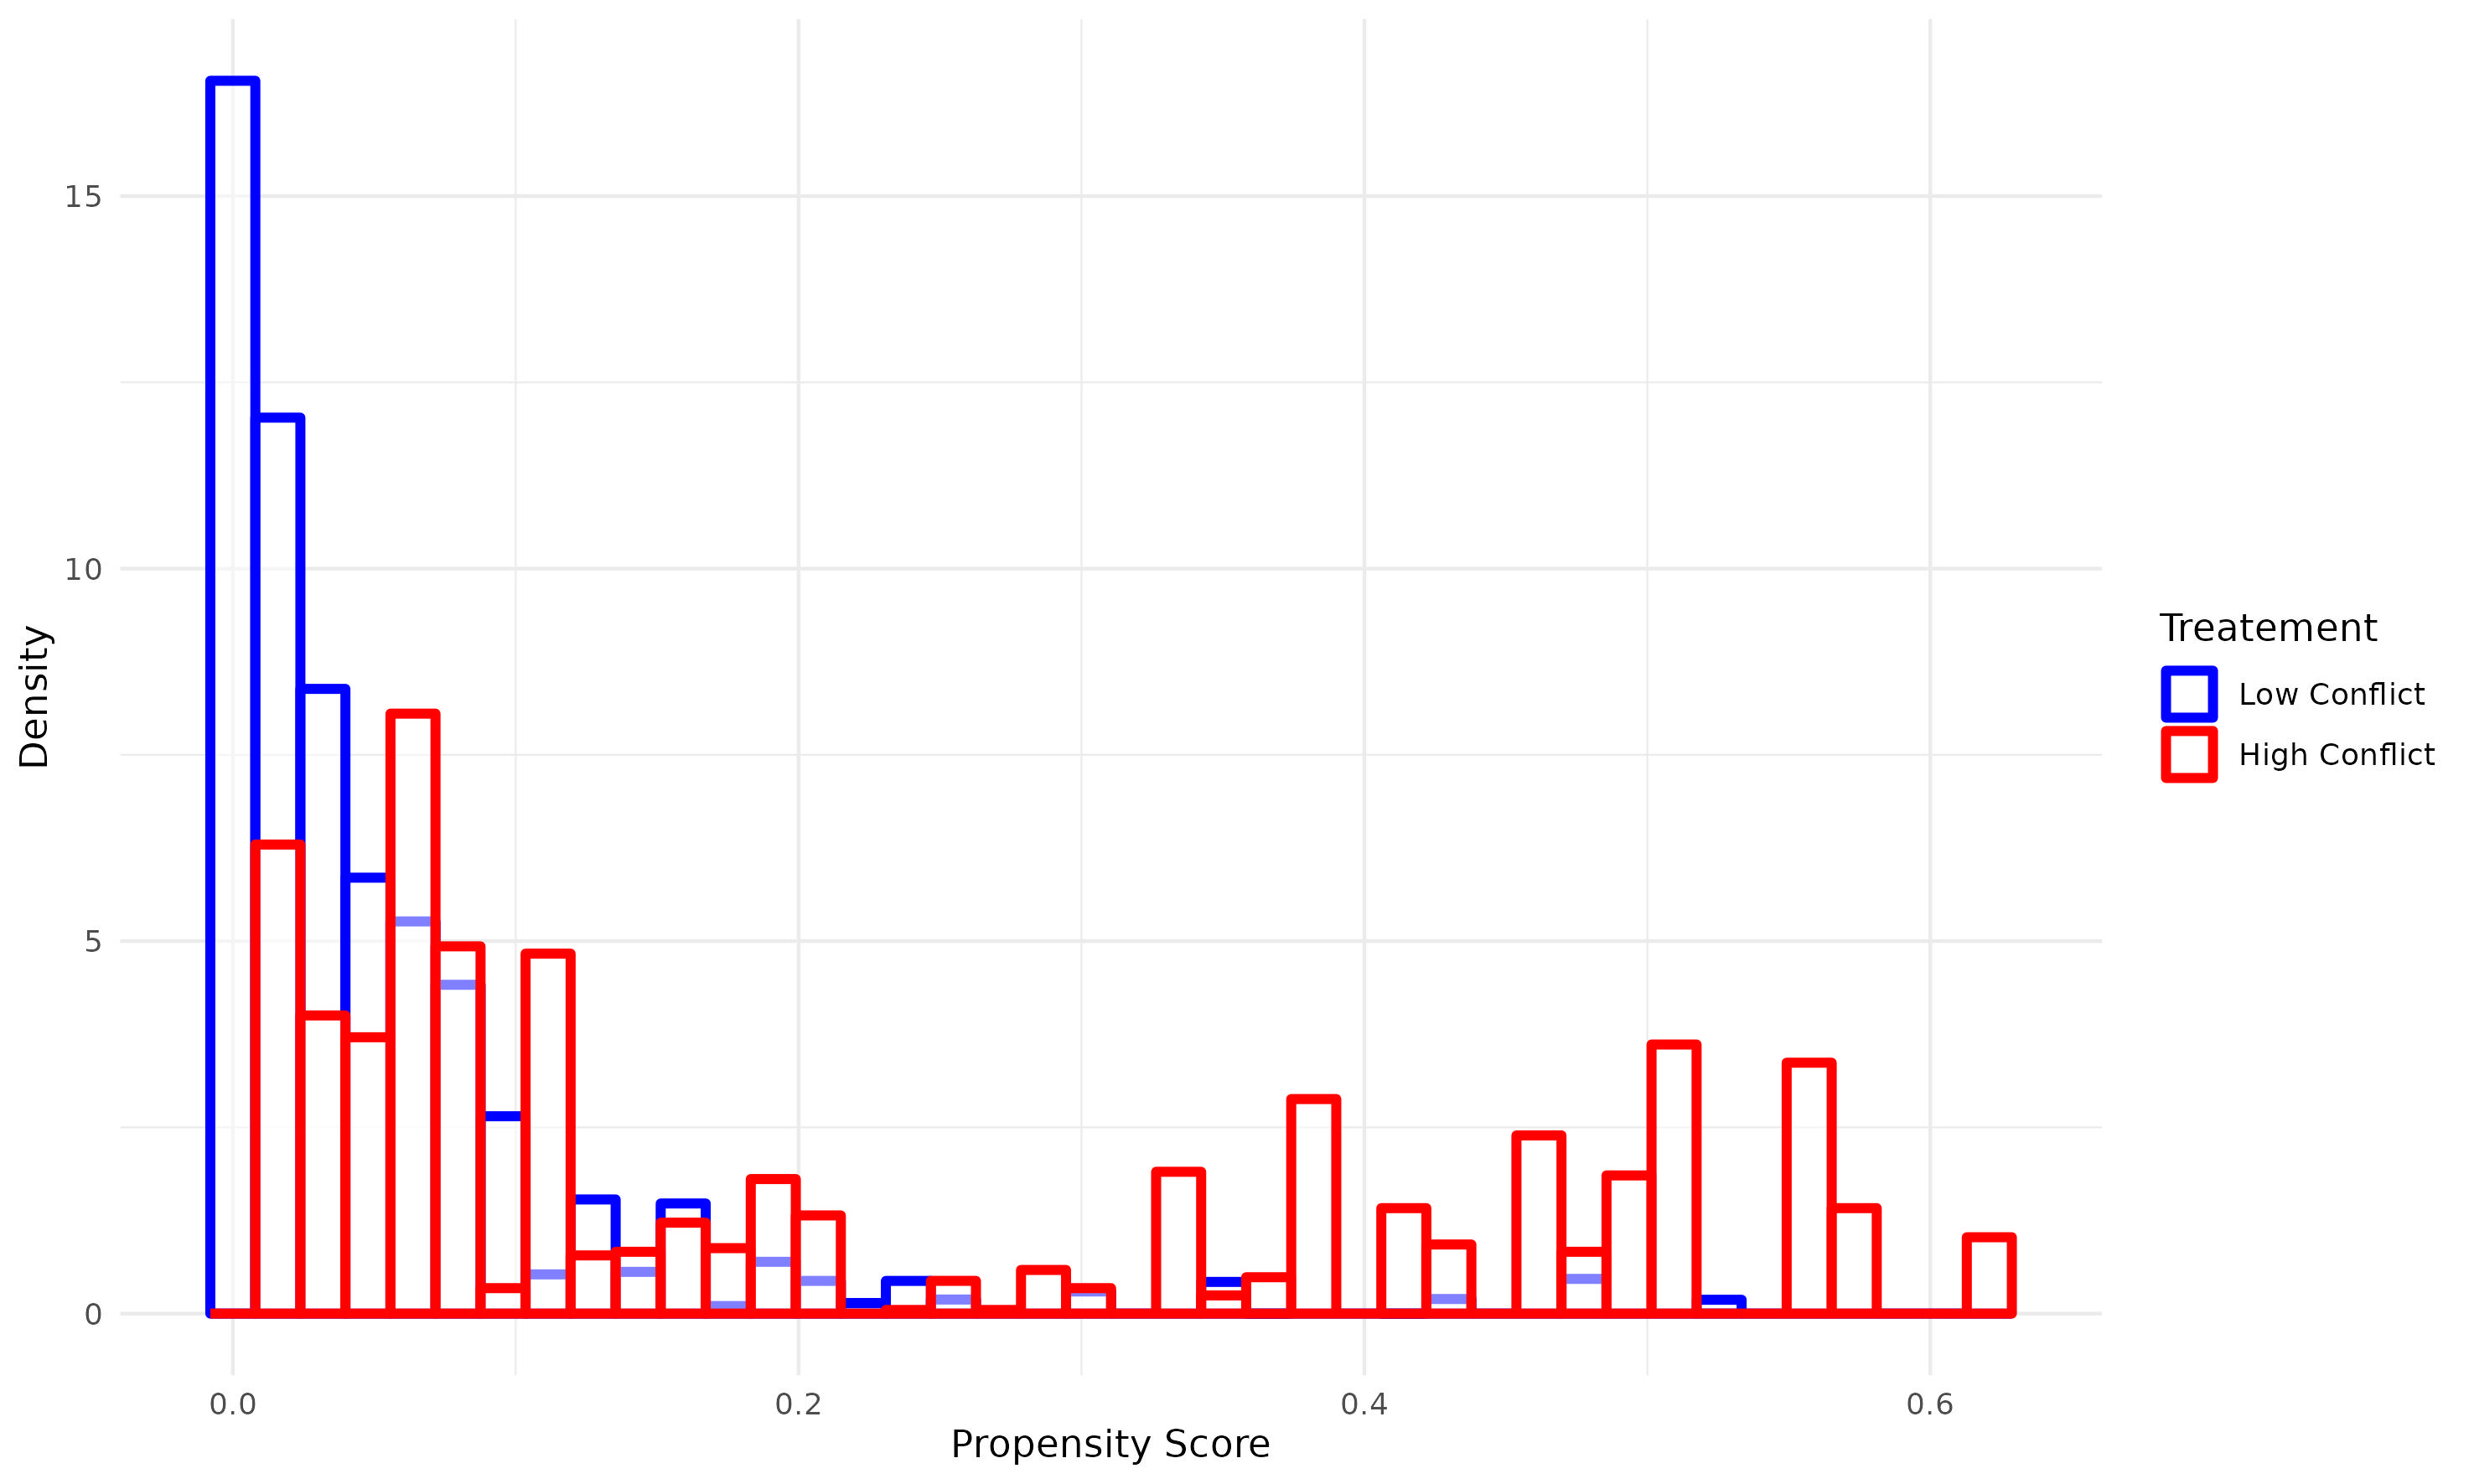
\includegraphics[width=0.8\textwidth]{../Analysis files/ps_overlap.jpg}
\caption{This figure shows the distribution of propensity scores for low and high-conflict regions, based on regression from Table 8.}
\label{fig:ps_overlap}
\end{figure}


% TODO : Overall DRDiD Estimate Results.
% TODO : Migration Controlled DRDiD Estimate Results.

% TODO : Gulmi vs Arghakhanchi showdown.

\section{Estimates}

Table 9 reports the Doubly Robust DiD\footnote{All estimates are calculated using the \textit{drdid} package from \textcite{sant2020doubly}. For documentation and use, see \url{https://psantanna.com/DRDID/}} estimates for five outcome variables.
Being in a high-conflict district has no effect on a person's status of being usually employed(employed for more than six months in the past year). We do see negative employment effects on short-term employment metrics like the status of being currently-employed or currently-self employed (pertaining to the reference period of last 7 days). More importantly, conflict intensity has a large
negative effect on an individual's work hours, with individuals in high conflict-afflicted regions estimated to work $4.7$ hours less on average than the comparison group. This is a decrease in $-0.18$ standard deviations on the standardize scale. There is likewise a $-4.29$ hours effect on self-employment, a $0.17$ standard deviations decrease.

% latex table generated in R 4.1.2 by xtable 1.8-4 package
% Mon Sep  8 12:59:48 2025
\begin{table}[ht]
\centering
\begin{tabular}{rrrrr}
  \toprule
 & ATT & se & lci & uci \\ 
  \midrule
Usually Employed & 0.01 & 0.01 & -0.02 & 0.03 \\ 
  Currently Employed & -0.03 & 0.01 & -0.06 & -0.01 \\ 
  Currently Self-employed & -0.04 & 0.01 & -0.06 & -0.01 \\ 
  Work Hours & -4.67 & 0.88 & -6.40 & -2.94 \\ 
  Work Hours (std) & -0.18 & 0.04 & -0.25 & -0.12 \\ 
  Self Employment Hours & -4.29 & 0.92 & -6.10 & -2.48 \\ 
  Self Employment Hours (std) & -0.17 & 0.04 & -0.25 & -0.10 \\ 
   \bottomrule
\end{tabular}
\caption{Doubly Robust DiD estimates of ATT} 
\end{table}


\subsection{Accounting for Migration}
As discussed in the section \textit{Underlying Theory}, large swaths of people left conflict-heavy regions during the Civil War\parencite{insec2008}, especially after 2001 A.D. when violence escalated. Between 2002 and 2004, 50,365 people were displaced: 3,837 and 21,320 people by the state and the Maoists respectively, whereas 25,199 persons emigrated from fear and terror \parencite{lawoti2010maoist}. It is plausible to assume that those who managed to move from high to low-intensity areas were likely the ones with the means to do so. This means the NLFS 2008 data may not fully capture region-specific labor supply, since it is already shaped by migration. As a result, our DiD estimates could be biased.

To address this, Table 10 reports DiD estimates only for those who did not move between 1996 and 2008 A.D., whom we classify I permanent residents. I excluded people if:

\begin{itemize}
	\item They were not born in their current VDC/municipality, their last usual residence was elsewhere, and they migrated to the current place less than 12 years ago; or
	\item They were born in their current VDC/municipality, but had lived elsewhere, and returned less than 12 years ago.
\end{itemize}

Everyone else was treated as a permanent resident. The DiD estimates that account for migration are reported in Table 10.

% latex table generated in R 4.1.2 by xtable 1.8-4 package
% Thu Sep 18 16:11:31 2025
\begin{table}[ht]
\centering
\begin{tabular}{rrrrr}
  \toprule
 & ATT & se & lci & uci \\ 
  \midrule
Usually Employed & -0.00 & 0.01 & -0.03 & 0.02 \\ 
  Currently Employed & -0.04 & 0.01 & -0.07 & -0.02 \\ 
  Currently Self-employed & -0.05 & 0.01 & -0.07 & -0.02 \\ 
  Work Hours & -5.03 & 0.92 & -6.84 & -3.23 \\ 
  Work Hours (std) & -0.20 & 0.04 & -0.27 & -0.13 \\ 
  Self Employment Hours & -4.65 & 0.97 & -6.54 & -2.76 \\ 
  Self Employment Hours (std) & -0.19 & 0.04 & -0.26 & -0.11 \\ 
   \bottomrule
\end{tabular}
\caption{Doubly Robust DiD estimates
             of ATT accounting for migration} 
\end{table}


Results in Table 10 are consistent with, and in fact show stronger negative effects than, those in Table 9: individuals in high-conflict areas are even less likely to be usually or currently employed. There are similar negative effects on the number of hours worked.
% Bernoulli Employed Coefficient Plots
\begin{figure}[H]
	\centering
	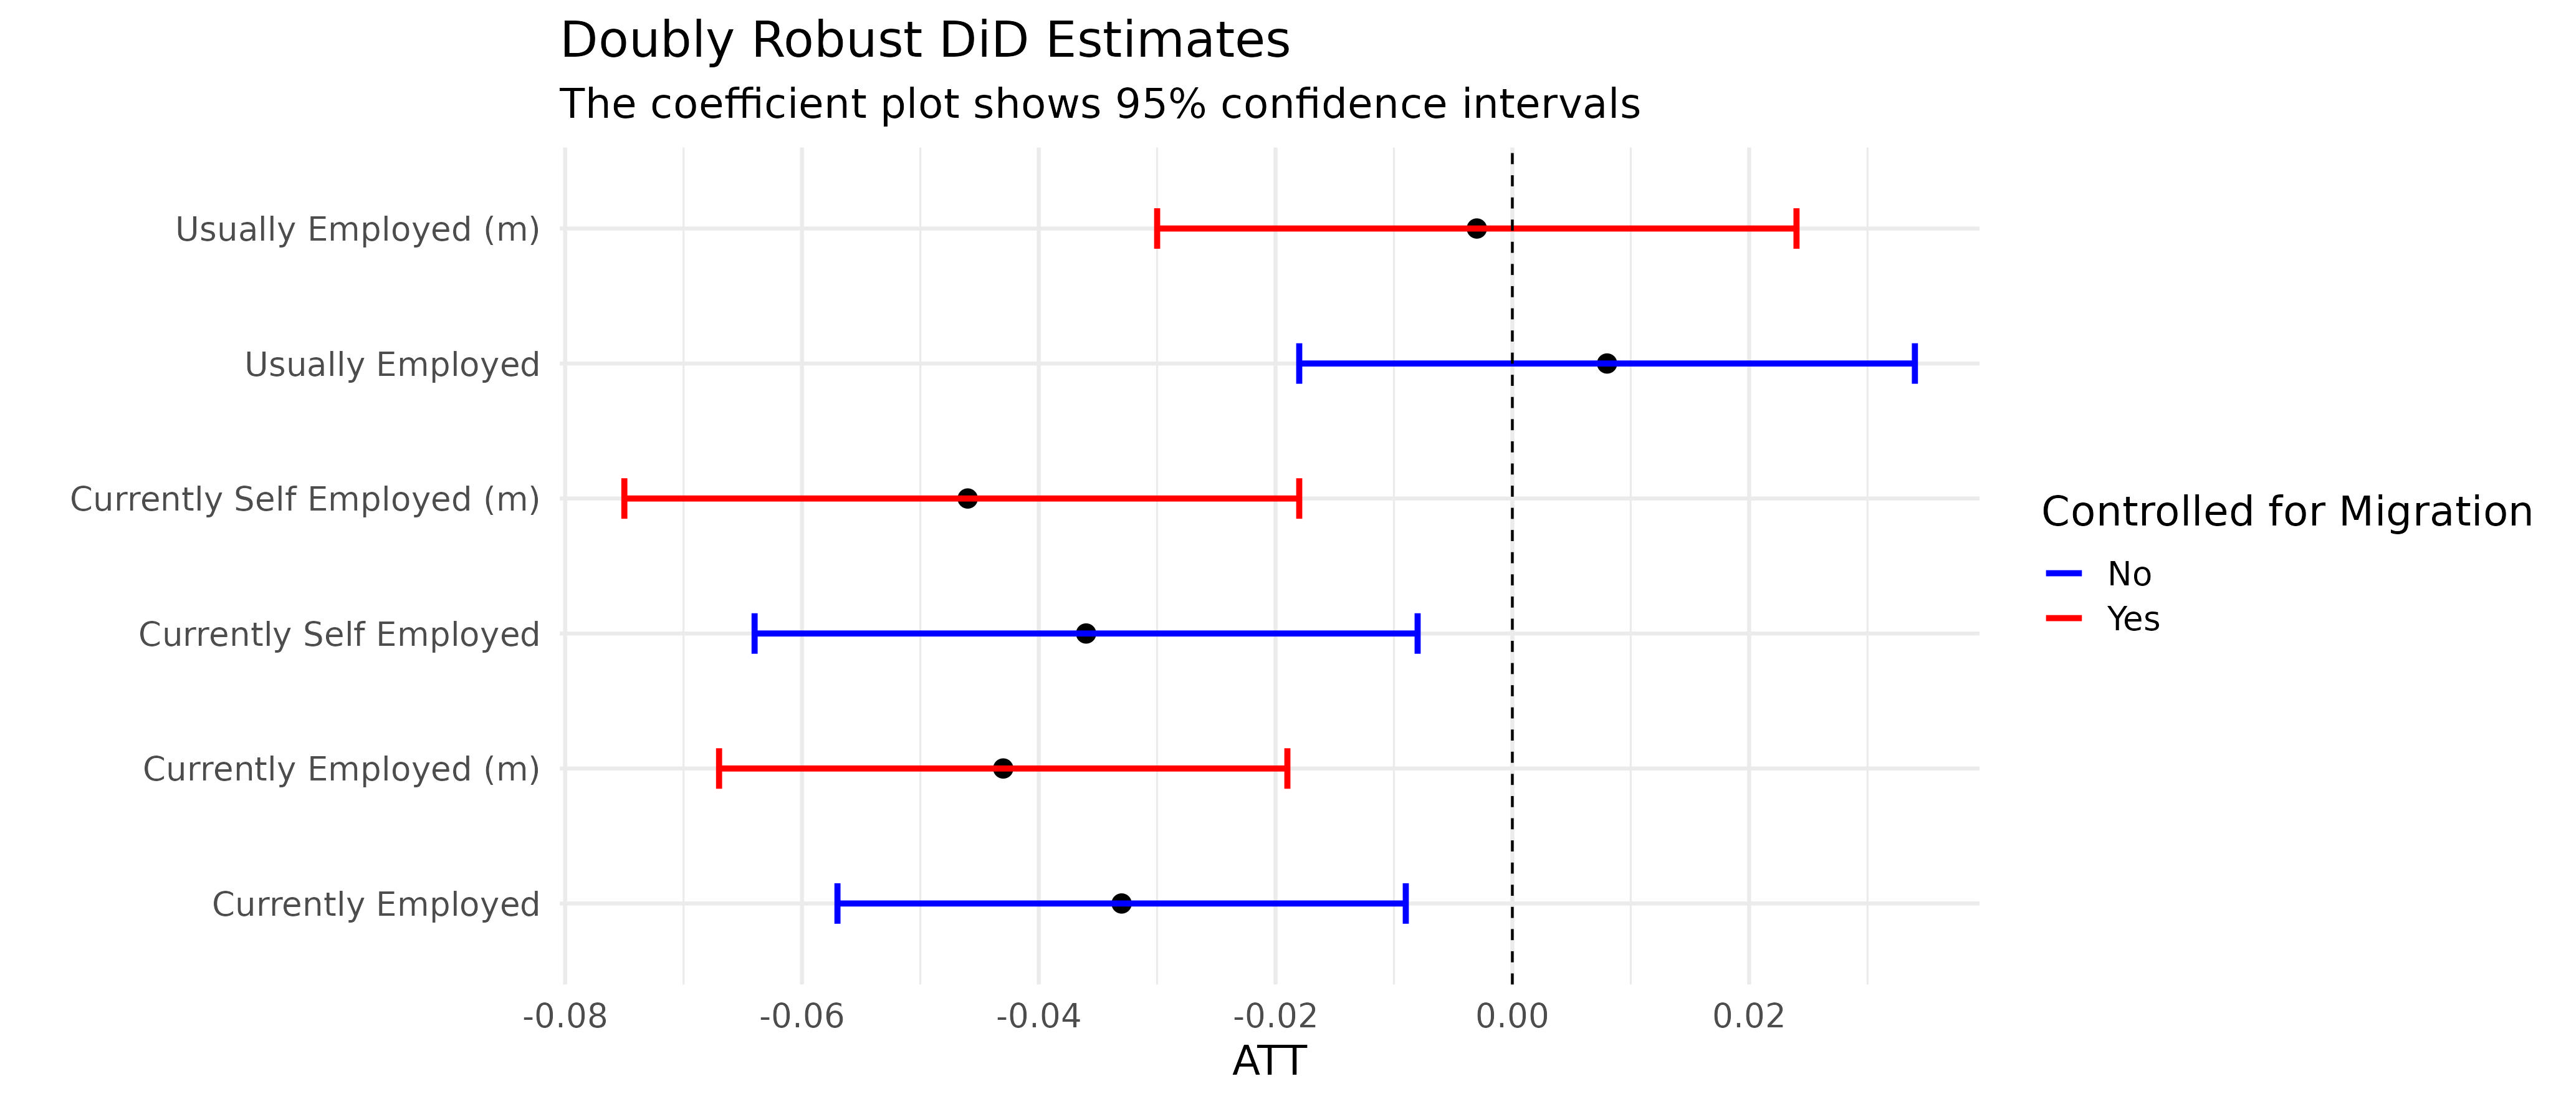
\includegraphics[width=1\textwidth]{../Analysis files/coefplot_1.jpg}
	\caption{Coefficient plot for three employment status outcome variables classified by whether the model accounted for migration. The point estimates are the estimates from DRDID and the error bars show 95 \% confidence intervals.}
	\label{fig:coefplot_1_1}
\end{figure}


% Work Hours Coefficient Plots
\begin{figure}[H]
	\centering
	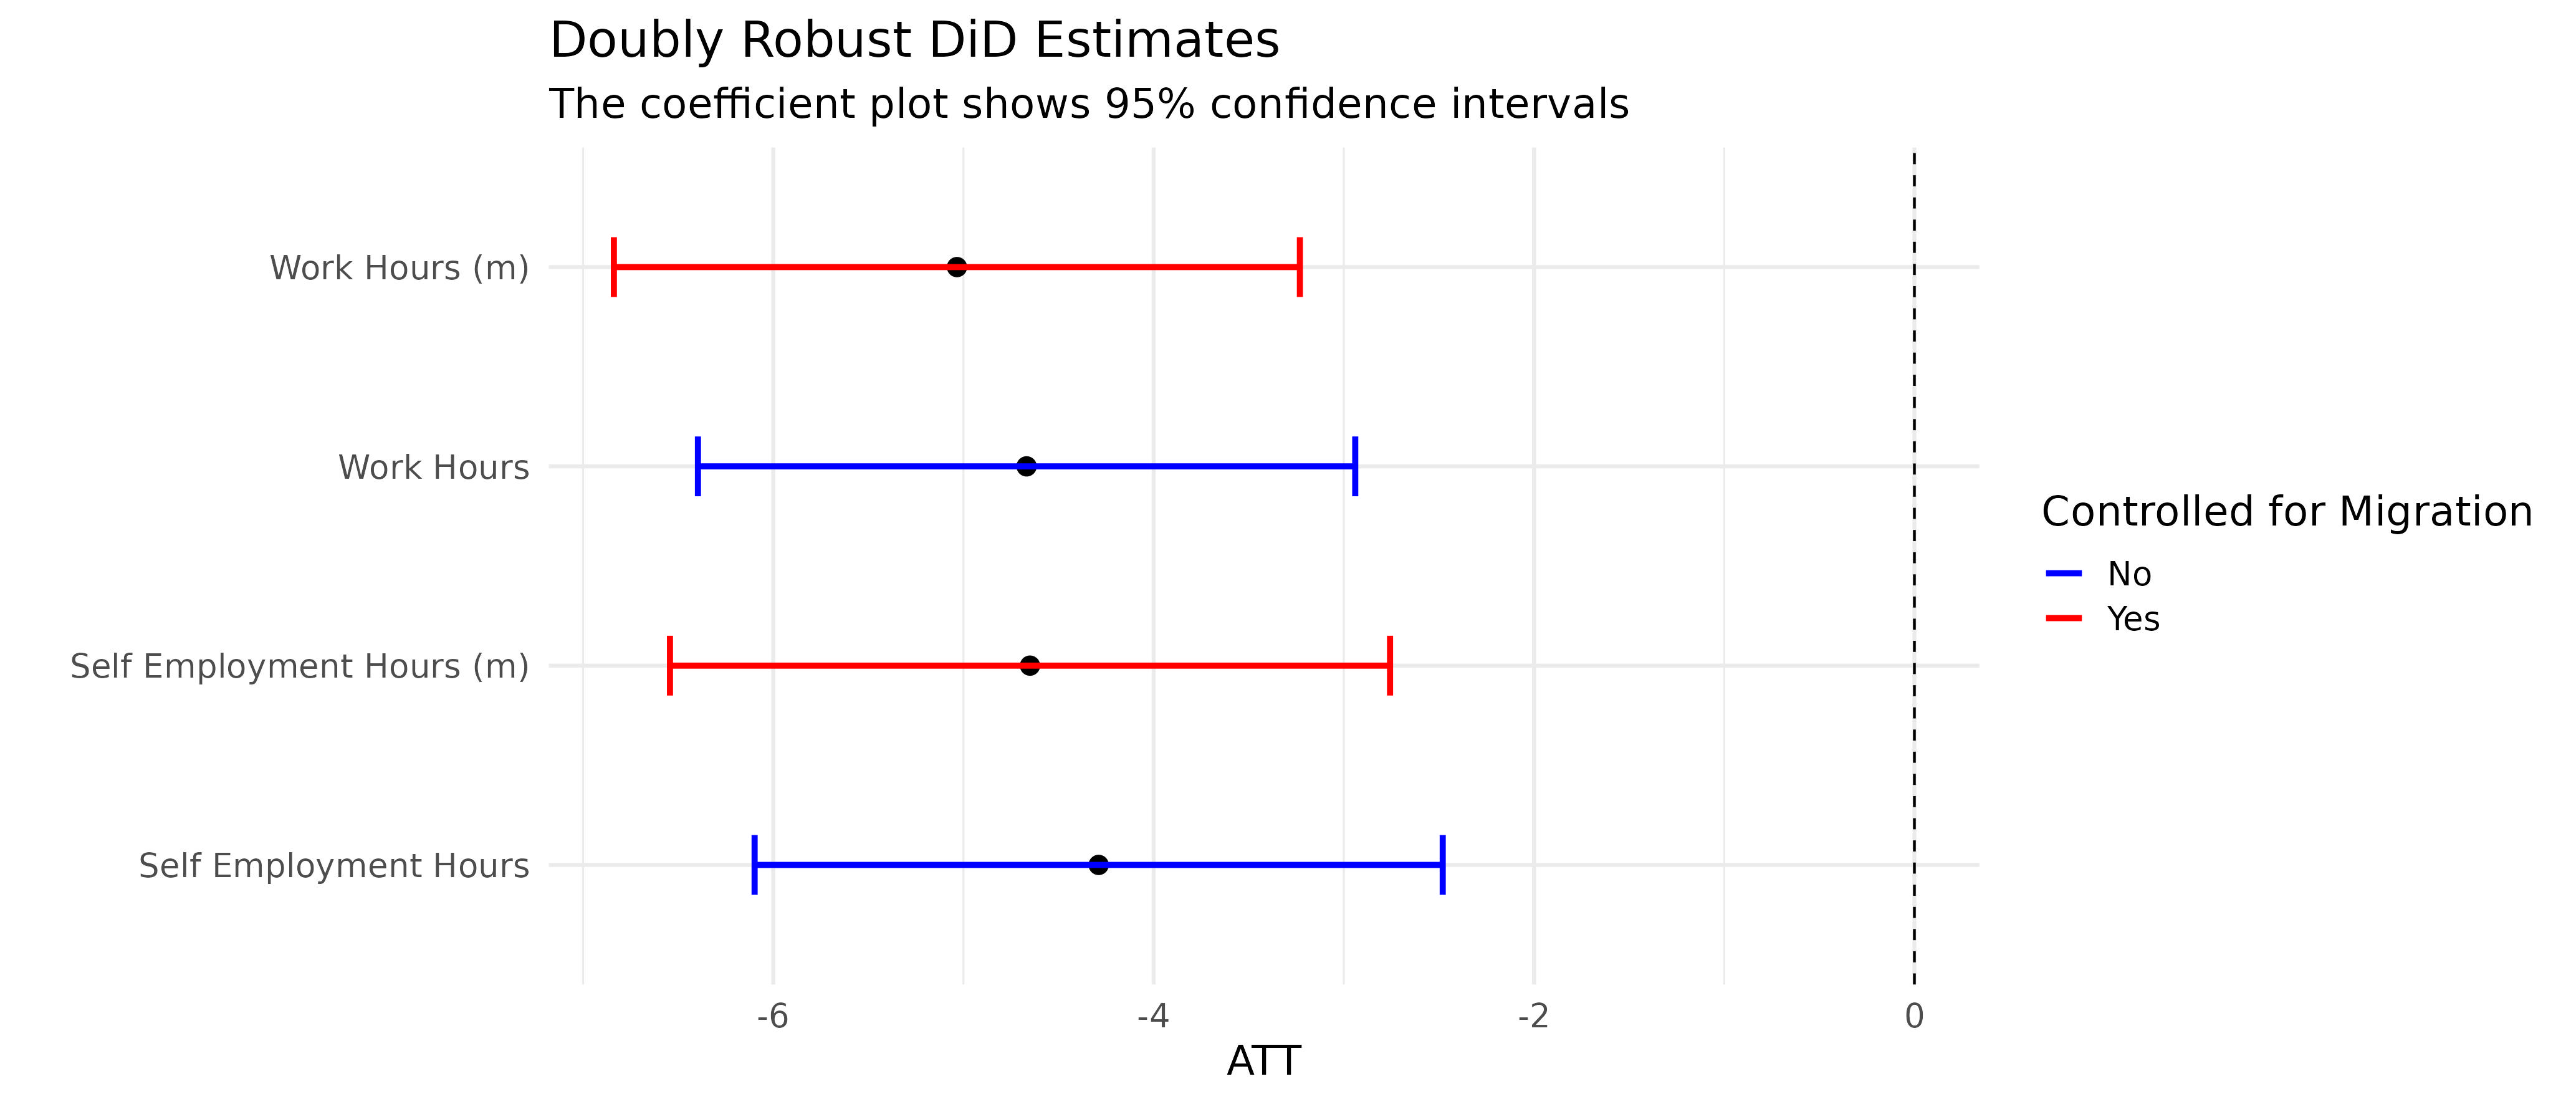
\includegraphics[width=1\textwidth]{../Analysis files/coefplot_2.jpg}
	\caption{Coefficient plot for two continuous outcome variables classified by whether the model accounted for migration. The point estimates are the estimates from DRDID and the error bars show 95 \% confidence intervals.}
	\label{fig:coefplot_1_2}
\end{figure}


\subsection{Seasonal Decomposition}
Work hours and the probability of employment depends of upon seasonal characteristics in an agricultural country like Nepal (more so during the 90s and the 2000s). Paddy, which is grown mostly in the Terai plains, is labor intensive during the monsoon months of Ashadh and Shrawan and in the harvesting month of Ashwin and Kartik. Winter and Dry seasons are amenable to various temperate fruits, vegetables and cash crops, such as cauliflowers, apples, wheat and tea. Such temporal differences in the need for labor-intensive employment is relevant because conflict in Nepal originated and afflicted districts in the Hill and the Mountainous belt more than districts in the Terai Belt\parencite{do2010geography}. This means that our earlier estimation of ATT only estimates an aggregate year-round effect of high-conflict. Decomposition of the ATT for rainy, winter and dry sub-samples of the NLFS dataset may provide us better insight into the mechanism through which conflict affects the labor supply.

Fortunately, both NLFS I and II were spread out over an entire year to allow us to capture such seasonal variations. The allocation of months to seasons for both NLFS I and NLFS II is given below:

\begin{table}[ht]
	
	\caption{Allocation of Months to Seasons for the NLFS}
	\renewcommand{\arraystretch}{1.2}
	\vspace{1em}
	\centering{}%
	\begin{tabular}{|c|c|c|c|}
		\hline
		\textbf{Season} & \textbf{Characteristic}& \textbf{Nepalese Calendar} & \textbf{Western Calendar}\\
		\hline
		1& Rainy & Jestha, Ashadh, Shrawan, Bhadra & mid-May to mid-Sep\\
		\hline
		2& Dry & Ashwin, Kartik, Mangsir, Poush & mid-Sep to mid-Jan \\
		\hline
		3& Winter & Magh, Falgun, Chaitra, Baisakh &  mid-Jan to mid-May\\
		\hline
	\end{tabular}
\end{table}

I partition the dataset into dry, winter, and rainy-only sample. This is done for two reasons:

\begin{enumerate}
	\item To decompose the ATT for dry, winter and rainy seasons.
	\item The untreated counter factual for treated units is more plausible within each sub sample.
\end{enumerate}


\subsubsection{Results: Dry Season (mid-Sep to mid-Jan)}
% latex table generated in R 4.1.2 by xtable 1.8-4 package
% Fri Sep 19 11:58:17 2025
\begin{table}[ht]
\centering
\begin{tabular}{rrrrr}
  \toprule
 & ATT & se & lci & uci \\ 
  \midrule
Usually Employed & -0.05 & 0.02 & -0.10 & -0.00 \\ 
  Currently Employed & -0.06 & 0.02 & -0.10 & -0.01 \\ 
  Currently Self-employed & -0.06 & 0.03 & -0.12 & -0.01 \\ 
  Work Hours & -4.21 & 1.53 & -7.21 & -1.21 \\ 
  Work Hours (std) & -0.17 & 0.06 & -0.28 & -0.05 \\ 
  Self Employment Hours & -4.03 & 1.56 & -7.09 & -0.97 \\ 
  Self Employment Hours (std) & -0.16 & 0.06 & -0.29 & -0.04 \\ 
   \bottomrule
\end{tabular}
\caption{Doubly Robust DiD estimates of ATT (Dry Season)} 
\end{table}

For dry seasons, the negative employment effect matches the overall negative effect of 4 to 5 less work hours. There is however lower average probability of being currently or usually employed (note : the standard errors are bigger, likely due to lower N for each season-specific sub-sample)


\subsubsection{Results: Winter Season (mid-Jan to mid-May)}
% latex table generated in R 4.1.2 by xtable 1.8-4 package
% Fri Sep 19 11:58:17 2025
\begin{table}[ht]
\centering
\begin{tabular}{rrrrr}
  \toprule
 & ATT & se & lci & uci \\ 
  \midrule
Usually Employed & 0.08 & 0.02 & 0.03 & 0.12 \\ 
  Currently Employed & 0.04 & 0.02 & -0.00 & 0.08 \\ 
  Currently Self-employed & 0.07 & 0.02 & 0.03 & 0.12 \\ 
  Work Hours & 2.26 & 1.52 & -0.71 & 5.24 \\ 
  Work Hours (std) & 0.09 & 0.06 & -0.03 & 0.21 \\ 
  Self Employment Hours & 5.42 & 1.60 & 2.28 & 8.56 \\ 
  Self Employment Hours (std) & 0.22 & 0.07 & 0.09 & 0.34 \\ 
   \bottomrule
\end{tabular}
\caption{Doubly Robust DiD estimates of ATT (Winter Season)} 
\end{table}


For the winter season, the average employment effect is positive but only for those whose work could be categorized as self-employment. There is also higher average probability of being self-employed. However, the effect on overall work-hours (which is inclusive of self-employment work hours) is not statistically different from zero effect. 

Likely Explanation:
\begin{itemize}
	\item High conflict districts were mostly part of Nepal's hilly and mountainous belt. This means that their work cycle may not have followed the Jestha(mid-May) to Kartik(mid-October) paddy cycle of the agricultural Terai. Agriculture in the Hilly and Mountainous belt produce important cash crops and vegetables in the winter period. This maybe a reason why we see positive discrepancy in work hours and employment probability. 
\end{itemize}


\subsubsection{Results: Rainy Season (mid-May to mid-Sep)}
% latex table generated in R 4.1.2 by xtable 1.8-4 package
% Fri Sep 19 11:58:17 2025
\begin{table}[ht]
\centering
\begin{tabular}{rrrrr}
  \toprule
 & ATT & se & lci & uci \\ 
  \midrule
Usually Employed & -0.03 & 0.02 & -0.07 & 0.02 \\ 
  Currently Employed & -0.07 & 0.02 & -0.11 & -0.04 \\ 
  Currently Self-employed & -0.11 & 0.02 & -0.15 & -0.07 \\ 
  Work Hours & -8.52 & 1.46 & -11.38 & -5.65 \\ 
  Work Hours (std) & -0.34 & 0.06 & -0.45 & -0.22 \\ 
  Self Employment Hours & -11.29 & 1.53 & -14.30 & -8.28 \\ 
  Self Employment Hours (std) & -0.46 & 0.06 & -0.58 & -0.33 \\ 
   \bottomrule
\end{tabular}
\caption{Doubly Robust DiD estimates of ATT (Rainy Season)} 
\end{table}


We see the largest negative effect in the rainy season, with average negative employment effect of 8.5 hours for overall work, and 11 less work hours for work categorized as self-employment.




\section{Robustness}
There are some methodological and inferential concerns with the doubly robust DiD estimates in our setting:

\begin{enumerate}
	\item Districts are split into high- and low-conflict groups based on conflict deaths per 10,000 people (above the 75th percentile = high conflict). This cutoff creates an artificial boundary, so districts with very similar conflict levels can end up in different groups.
	\item Standard errors are estimated at the individual level, which means that everyone in a high-conflict region is treated as having the same exposure. This ignores district-level shocks, which is the actual source of variation \parencite{bertrand2004much}.
\end{enumerate}
While the inclusion of covariates help address potential parallel trends bias, a smaller-sample design-based analysis may address afore-mentioned concerns. For this purpose, I compare two-adjacent districts in Nepal -- Gulmi and Argakhanchi -- that are likely to be similar in covariates but differ considerably in conflict exposure as outlined in Table 11.

\begin{table}[H]
	\caption{Gulmi and Argakhanchi Conflict Deaths per 10,000 people}
	
	\renewcommand{\arraystretch}{1.2}
	\vspace{1em}
	\centering{}%
	\begin{tabular}{c|c|c}
		& 1998 (pre-period) & 2008 (post-period)\tabularnewline
		\hline 
		Gulmi $d_{L}$ & $0$ & $1.92$\tabularnewline
		Argakhanchi $d_{H}$ & $0$ & $11.7$\tabularnewline
		\hline 
	\end{tabular}
\end{table}

The choice of Gulmi and Arghakhanchi as comparison groups is based on two reasons:

\begin{enumerate}
	\item Neither district had any casualties by 1998, but conflict deaths in Arghakhanchi rose sharply over time, reaching high levels by the end of the conflict (see Table 11).
	
	\item Both districts lie in the western hills of Nepal and share similar ethnicity, culture, religion, and lifestyle. They are also likely to be similar in covariates by 1998, as shown in Table 12.
\end{enumerate}

% latex table generated in R 4.1.2 by xtable 1.8-4 package
% Fri Sep 12 07:55:58 2025
\begin{table}[ht]
\centering
\begin{tabular}{rrrr}
  \toprule
 & Norm. Diff & Treated Mean & Control Mean \\ 
  \midrule
Age & -0.05 & 31.82 & 32.49 \\ 
  Years of Education (All) & -0.03 & 3.19 & 3.30 \\ 
  Years of Education (If attended school) & -0.02 & 6.60 & 6.65 \\ 
  Hindu (1/0) & -0.40 & 0.91 & 0.99 \\ 
  Brahmin/Chhetri(1/0) & 0.11 & 0.54 & 0.49 \\ 
  Male & 0.03 & 0.36 & 0.35 \\ 
  Married & 0.14 & 0.77 & 0.70 \\ 
  Household Size & -0.22 & 5.06 & 5.49 \\ 
  Urban &  & 0.00 & 0.00 \\ 
  Ever Attended School & -0.02 & 0.49 & 0.50 \\ 
   \bottomrule
\end{tabular}
\caption{Covariate Balance Statistics} 
\end{table}

% TODO: Change the Caption for this Table in R.

As shown in Table 12, Gulmi and Arghakhanchi were very similar in key covariates in 1998, with only small differences in the share of the Hindu population. Similarly, Table 13 indicates no outstanding differences in their covariate trends over time. This evidence suggests that any violation of the parallel trends assumption for Gulmi and Arghakhanchi is likely to be minimal, and a conventional Difference-in-differences analysis can be carried out.

% latex table generated in R 4.1.2 by xtable 1.8-4 package
% Tue Sep 16 08:50:54 2025
\begin{table}[ht]
\centering
\begin{tabular}{rrr}
  \toprule
 & Control trend & Treatment trend \\ 
  \midrule
Age & -0.82 & -0.04 \\ 
  Years of Education (All) & 2.36 & 2.07 \\ 
  Years of Education (If attended school) & 1.13 & 1.58 \\ 
  Hindu (1/0) & 0.00 & 0.09 \\ 
  Brahmin/Chhetri(1/0) & -0.04 & 0.02 \\ 
  Male & 0.05 & 0.01 \\ 
  Married & 0.00 & -0.08 \\ 
  Household Size & -0.25 & -0.27 \\ 
  Urban & 0.00 & 0.00 \\ 
  Ever Attended School & 0.23 & 0.15 \\ 
   \bottomrule
\end{tabular}
\caption{Covariate Balance Statistics for trends/differences (2008 - 1998)} 
\end{table}


To estimate the difference-in-differences, I use a Bayesian hurdle lognormal likelihood for the outcome variable \textit{Work Hours}. I choose a Bayesian approach for two main reasons:

\begin{enumerate}
	\item The distribution of Work Hours has a clear spike at zero, representing individuals who did not work. (See figure 4)
	\item Work Hours is naturally bounded at zero and cannot take negative values.
\end{enumerate}

The standard OLS DiD estimator does not restrict outcomes to positive values and cannot account for the probability of zeros. This is also true for doubly robust DiD methods, which rely on weighted least squares for outcome regression and inverse probability tilting for propensity scores. Since conditioning on covariates is not required in this setting, a Bayesian model with a hurdle lognormal likelihood for the outcome variable is appropriate.

\begin{figure}[H]
	\centering
	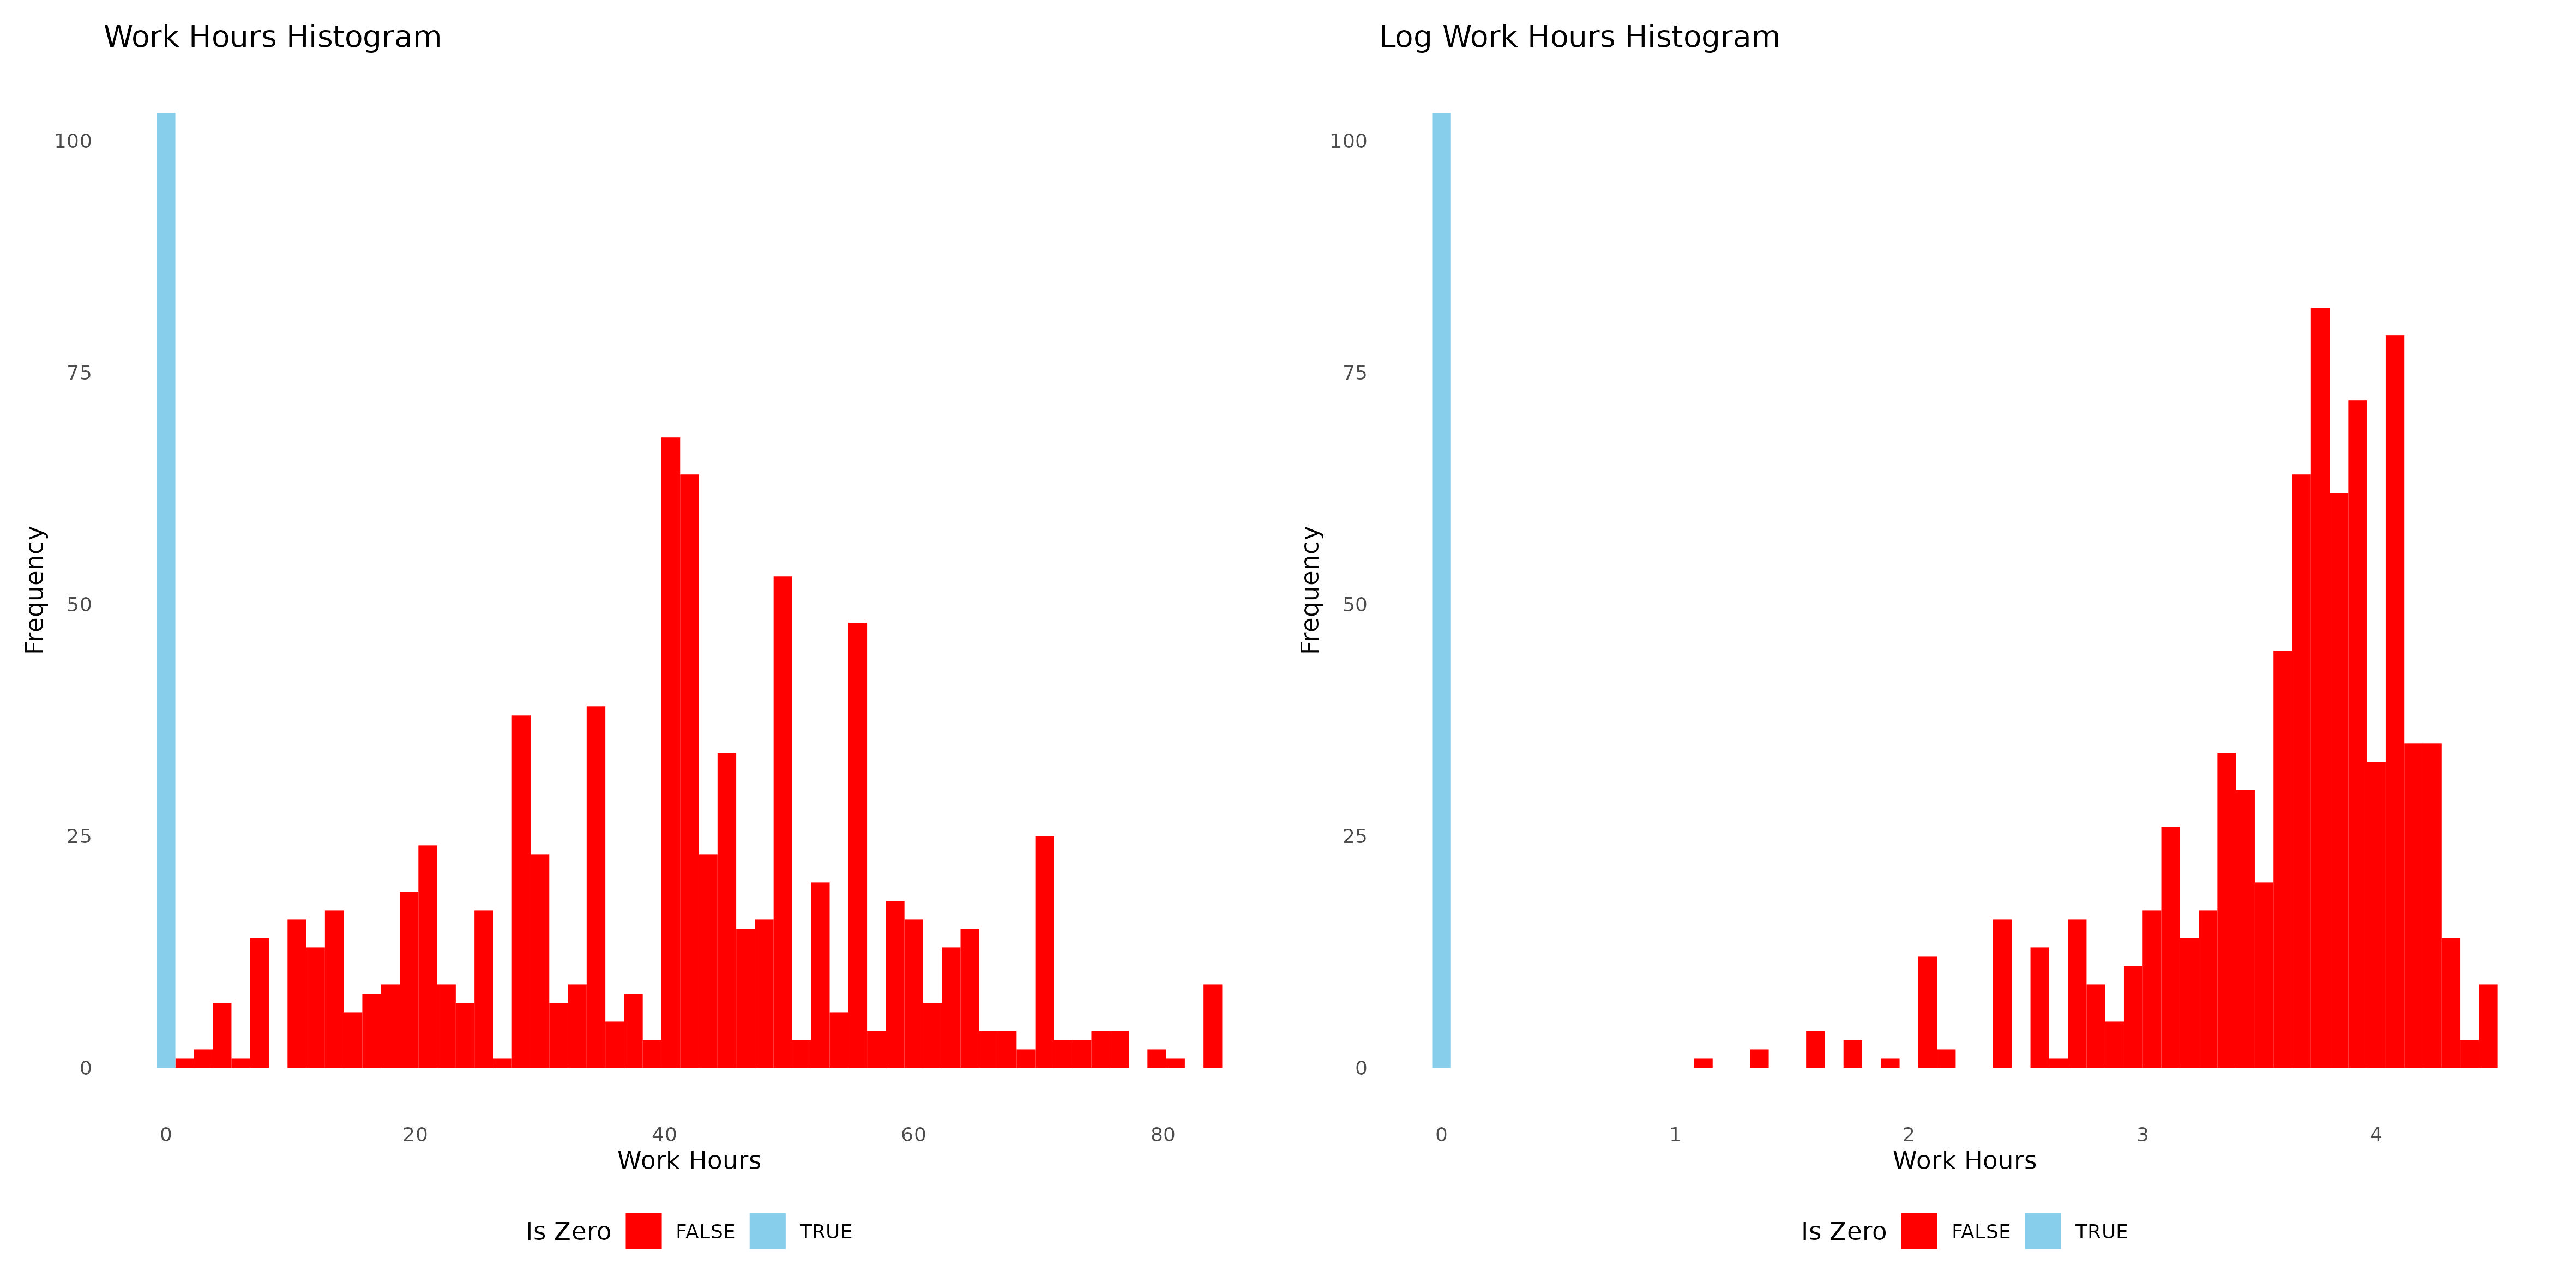
\includegraphics[width=1\textwidth]{../Analysis files/wh_histogram.jpg}
	\caption{Histogram of variable work hours; Left : in a standard scale. Right : In the log scale.}
	\label{fig:wh_histogram}
\end{figure}

The econometric model can be written as:
\begin{align*}
	wh_{i} \text{(work hours)} &\sim \text{hurdleLognormal}(hu_i, \mu_i) \\
	\mu_{i} &= \alpha_{GID[i]} \\
	hu_{i} &= \beta_{GID[i]} \\
	\alpha_{GID[i]} &\sim \text{Lognormal}(3,\, 0.5) \\
	\beta_{GID[i]} &\sim \text{Normal}(-1,\, 1)
\end{align*}

where, for $GID[i]$, $i = \{ 1, 2, 3, 4\}$ represents four interactions group ids: 1 = 1998 Gulmi (low-conflict); 2 = 1998 Arghakhanchi (high-conflict); 3 = 2008 Gulmi (low-conflict); 4 = 2008 Arghakhanchi (high-conflict).

Here, $\mu_i$ is the average work hours (conditional on work hours $> 0$) in the log scale, and $hu_i$ represents the probability of observing $0$ hours worked, which are estimated on the log and logit scales respectively.






\begin{figure}[H]
	\centering
	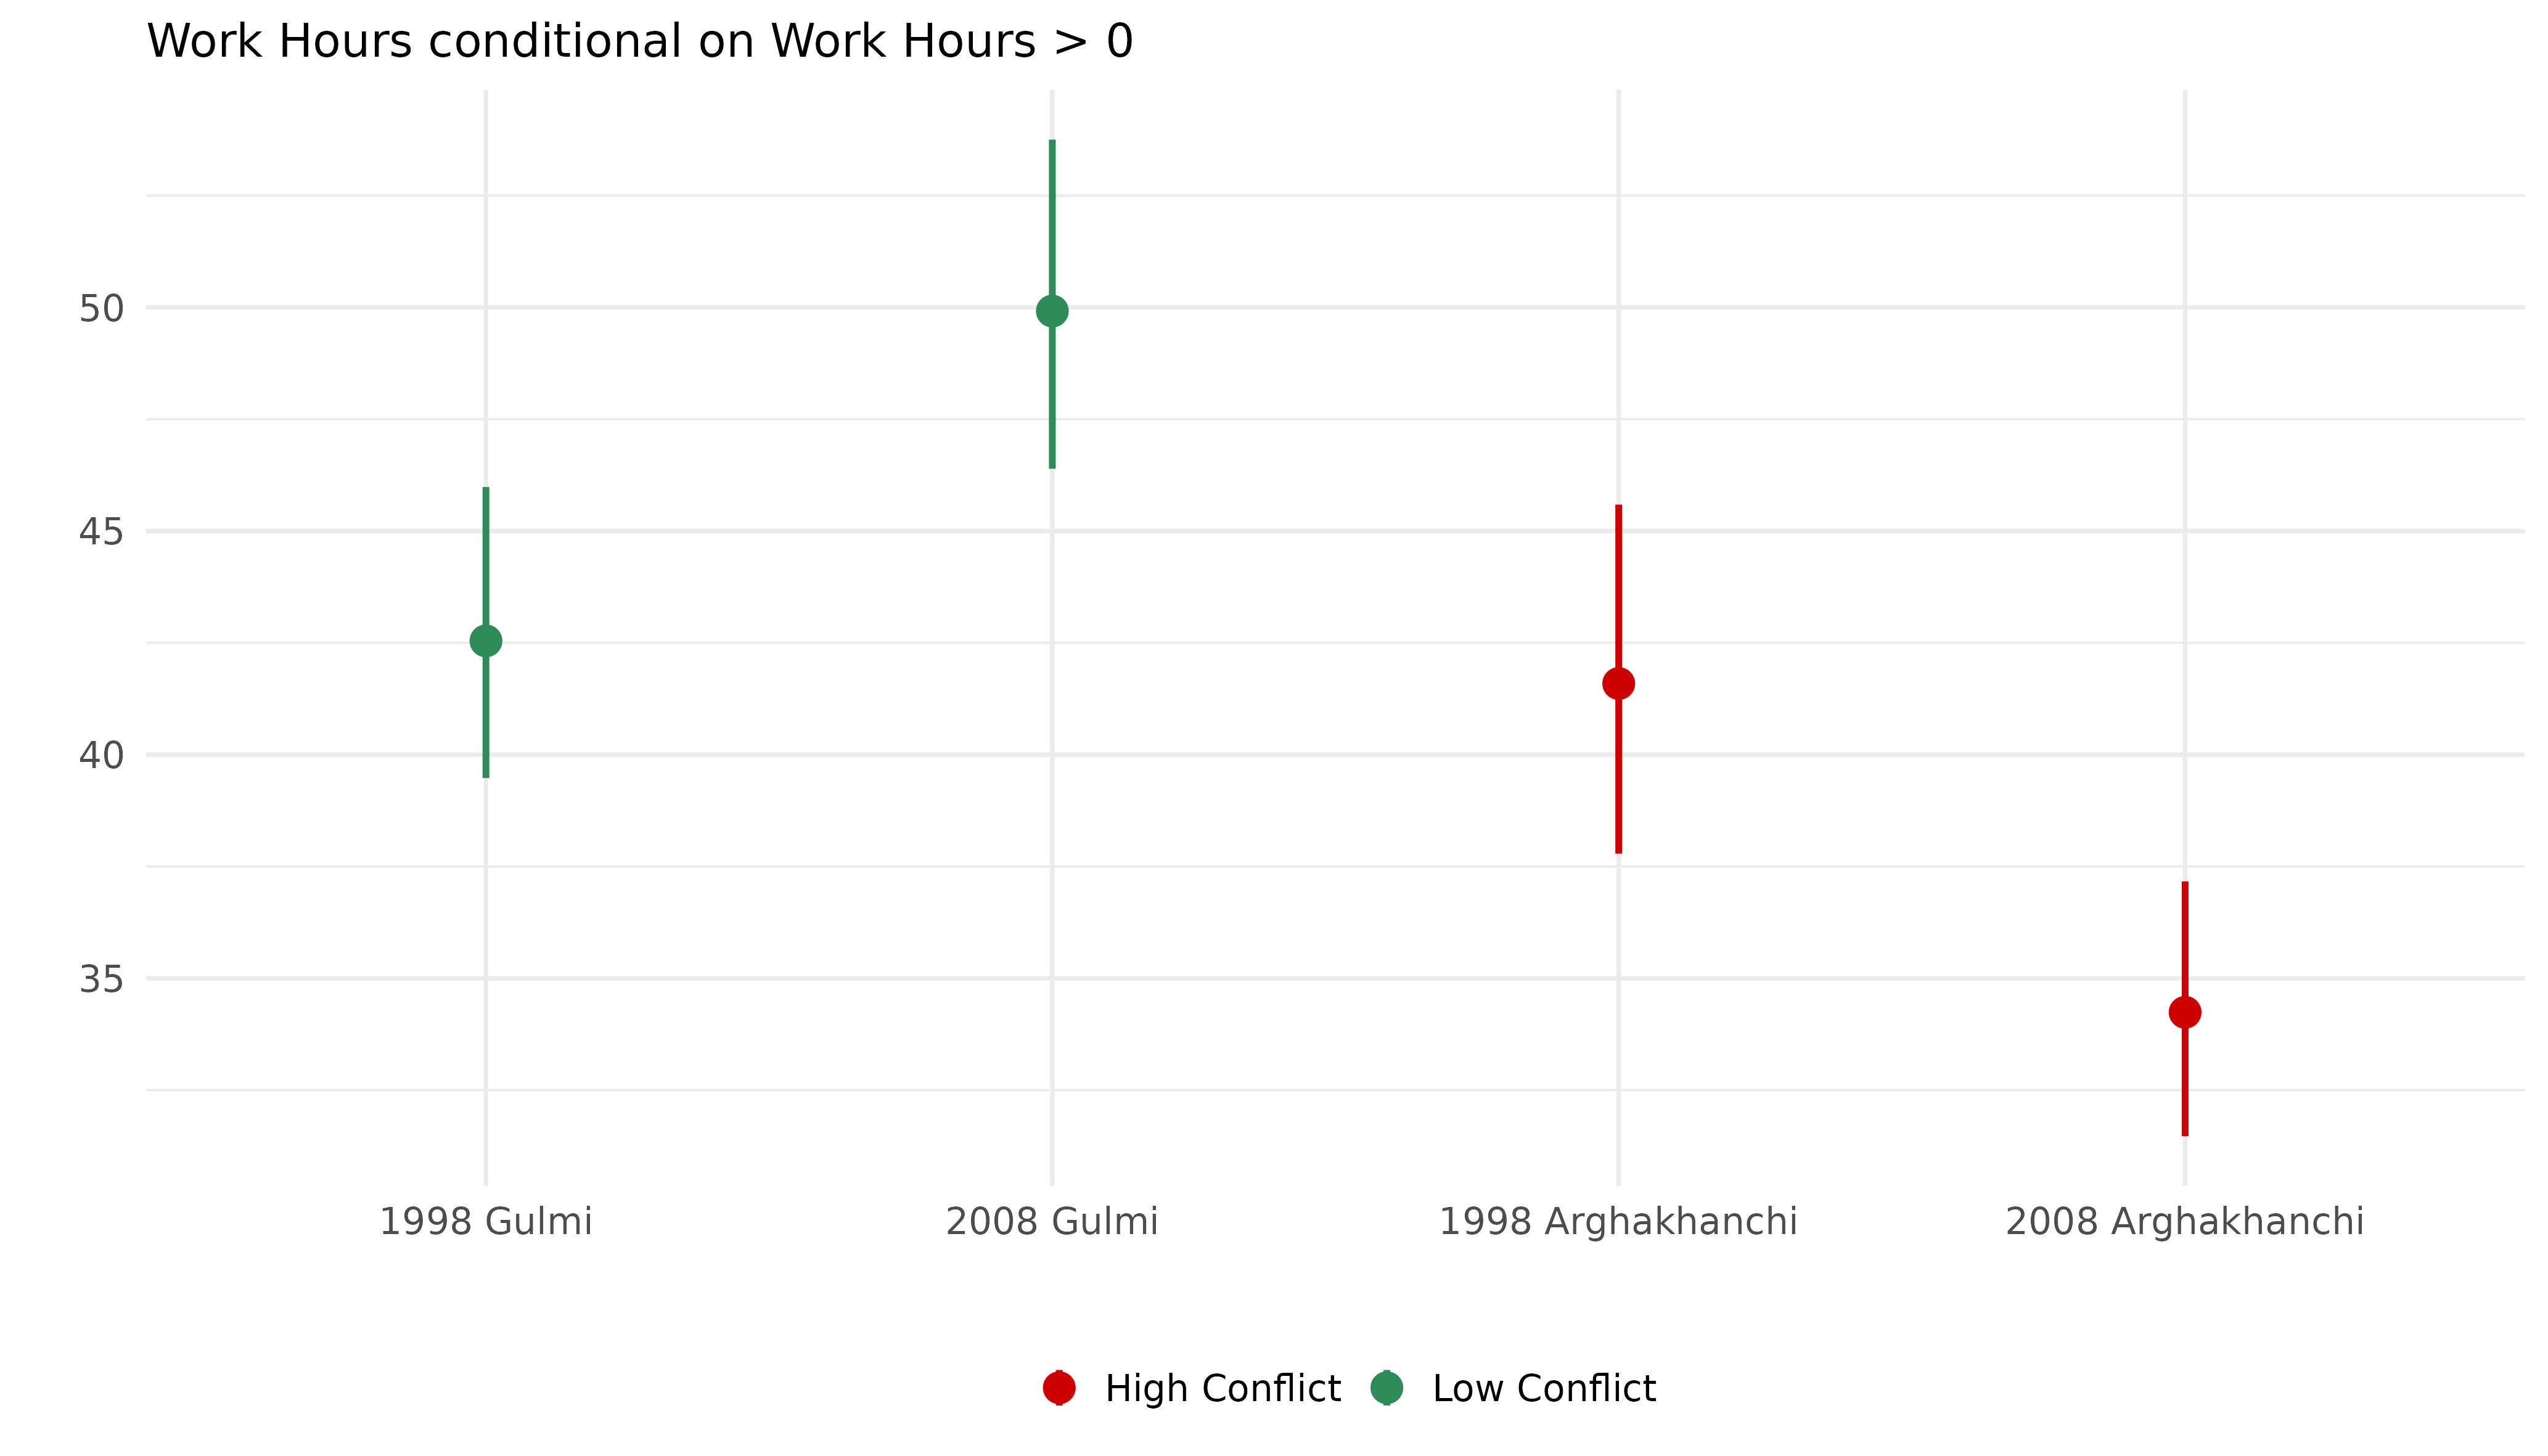
\includegraphics[width=1\textwidth]{../Analysis files/coefplot_map.jpg}
	\caption{The figure shows predicted non-zero work hours for each of the four interaction groups. Green shows the Bayesian prediction for low-conflict Gulmi and red shows the prediction for high-conflict Arghakhanchi before and after conflict.}
	\label{fig:coefplot_map}
\end{figure}

\begin{figure}[H]
	\centering
	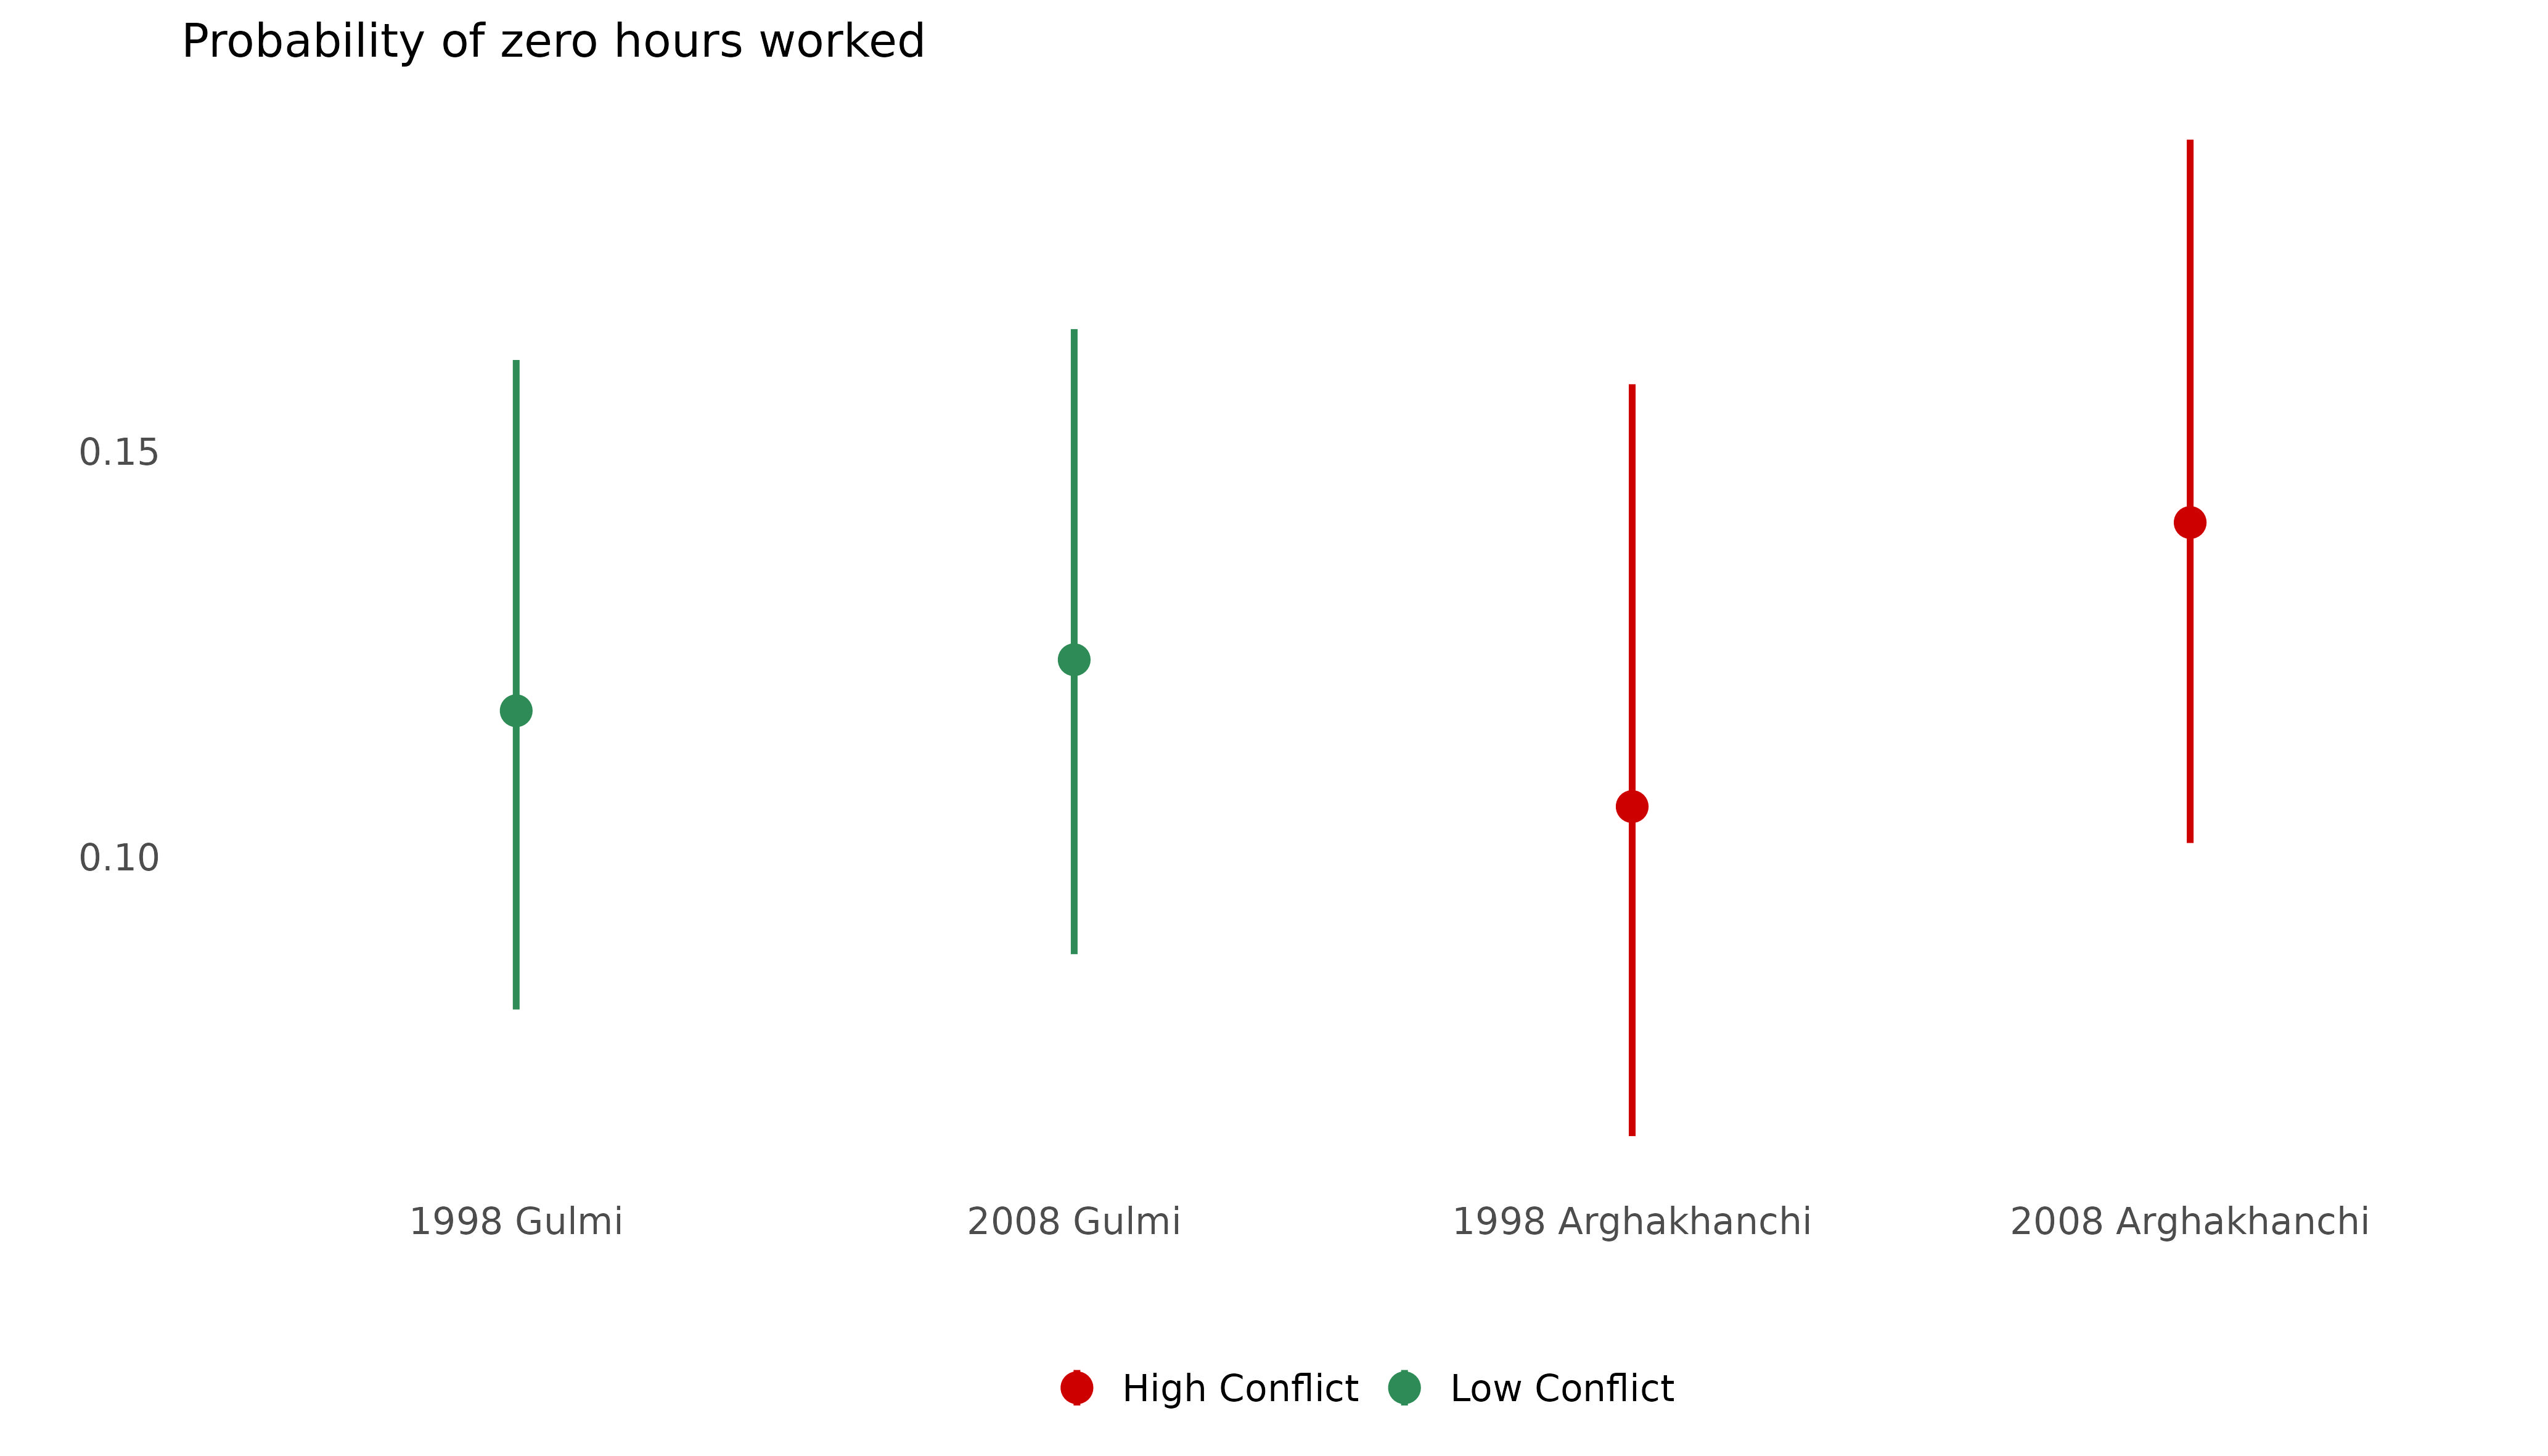
\includegraphics[width=1\textwidth]{../Analysis files/coefplot_map_hu.jpg}
	\caption{The figure shows predicted hurdle probability (probability of observing $0$ hours worked) for each of the four interaction groups. Green shows the Bayesian prediction for low-conflict Gulmi and red shows the prediction for high-conflict Arghakhanchi before and after conflict.}
	\label{fig:coefplot_map_hu}
\end{figure}

DiD Contrasts:

\begin{table}[H]
	\caption{Posterior Summary of DiD contrasts (credibility intervals width = $.95$)}
	
	\renewcommand{\arraystretch}{1.2}
	\vspace{1em}
	\centering{}%
	\begin{tabular}{c|c|c|c|}
		& Estimate & lci& uci \tabularnewline
		\hline 
		Work Hours & $-14.7$ & $-21.61$ & $-7.76$ \tabularnewline
		Probability of zero (hurdle) & $0.02$ & $-0.057$ & $0.11$ \tabularnewline
		\hline 
	\end{tabular}
\end{table}

The group-wise interaction for the two-district comparison shows that heavily affected Arghakhanchi saw a significant drop in work hours. The Difference-in-Difference contrast estimates an average of 14 reduced work hours. But, as shown in Figure 6 and Table 14, there is no change in the probability of working zero hours, that is, no effect on inactivity. This points to under-employment rather than outright unemployment.

The DiD contrast from this small two-district analysis is consistent with the large-sample results described earlier. While the size of the effect varies, the overall direction is the same: employment was negatively affected. In some heavily hit districts this meant unemployment, while in others it meant under-employment

\section{Discussion}
A decline in average work hours can result either from fewer people finding employment or from jobs requiring fewer hours, due to higher productivity or a shift toward types of work with lower time demands. Since the likelihood of being employed is largely unchanged, the more likely explanation is the latter.

A decline in working hours is not inherently negative. From a labor supply perspective, if individuals voluntarily choose to work fewer hours in response to higher wages, while keeping their preferences constant, this may reflect rising productivity and improving economic conditions. However, when reduced hours are involuntary, maybe due to a lack of full-time opportunities or declining economic activity, the implications become concerning. In the context of Nepalese Civil War, it's difficult to interpret reductions in work hours as voluntary adjustments amid infrastructure destruction and uncertainty. Rather, the decline likely reflects a forced contraction in the availability of work, made worse by limited mobility due to fear of violence. Similarly, as alluded by \textcite{blattman2010civil}, military experience is a poor substitute for education and labor market experience. The young conscripts in the Nepalese Civil War may find it harder to integrate themselves in the labor market with reduced high-level education and employment experience.

In terms of labor demand, being in a conflict-afflicted area is risky for firms, both in an economic sense of increased operational costs as well as the risk of physical danger. As a result, reduced investment, business closures, or relocation become plausible outcomes, which has negative effects on employment. On the other hand, if relatively underdeveloped, conflict-affected regions experienced convergence toward more developed, less-affected areas between 1998 and 2008, through shifts in industry composition, firm size, and labor demands, the productivity hypothesis cannot be ruled out.

% References	
\printbibliography
	
\end{document}
